\chapter{Programmation linéaire en nombres entiers mixtes de SMEPC}
\minitoc
\newpage
\label{MIP_3_plus}
\section{Introduction}
Ce chapitre présente la modélisation linéaire en nombres entiers qu'on a réalisé du problème SMEPC.
Dans la \textbf{section} \ref{Le modèle SMEPC}, on explique la problématique des travaux de recherche réalisés durant ce projet de thèse, à savoir la conception d'algorithmes et de modèles pour résoudre le problème de synchronisation de la production et des activités d'un véhicule autonome. On définit les données d'entrées et une solution d'une instance du problème \textbf{SMEPC}. La \textbf{section} \ref{extensions_SMEPC} liste les différentes extensions du problème \textbf{SMEPC}, qui seront considérées comme des perspectives éventuelles pour une extension de ce travail. La \textbf{section} \ref{modelisation_SMEPC} présente le modèle mathématique du problème \textbf{SMEPC} en présentant les variables, la fonction objectif et les contraintes du problème. La \textbf{section} \ref{SMEPC_model} présente le programme linéaire à variable mixte de SMEPC.  Dans la \textbf{section} \ref{sec4}, on présente la relaxation linéaire du programme précédent. %La \textbf{section} \ref{sec5} présente une approche branch and cut pour SMEPC.
 La \textbf{section} \ref{NP-hard_SMEPC} présente les résultats de complexité qu'on a obtenu,
 %on présente d'abord quelques généralités sur la complexité,
 puis, on démontre que le problème \textbf{SMEPC} est NP-difficile. On finit ce chapitre en présentant à la section \ref{num_MIP} les résultats expérimentaux.


\section{Le problème SMEPC : \textit{Synchronous Management of Energy Production and Consumption}}
\label{Le modèle SMEPC}
Dans cette partie, on explique le problème \textbf{SMEPC} : Synchronous Management of Energy Production and Consumption. Pour cela, on précise les données d'entrées de notre problème. Ensuite, on présente ce qu'est une solution d'une instance du problème \textbf{SMEPC}. Enfin, on explique les sous-problèmes qui émanent du problème \textbf{SMEPC}. 

\begin{figure}[H]
	\centerline{
		\includegraphics[height=9cm]{images_these/illustration_depotrond.pdf}}
	\caption[Le dépôt et la micro-usine]{ Le dépôt et la micro-usine.}
	\label{depot}
\end{figure}
Nous considérons ici un véhicule qui doit effectuer des tâches de logistique interne, tout en suivant un itinéraire $\Gamma$ qui commence et se termine sur une station particulière appelée \textit{Dépôt} illustré à la figure (\ref{depot}). Le véhicule parcourt les stations $j=1, \dots, M$, selon cet ordre. Cet itinéraire est appelé une tournée. La station de départ \textit{Dépôt} a l'étiquette $Depot=0$ et est appelé dépôt initial. La station de fin \textit{Dépôt} a l'étiquette $Depot=M + 1$ et est appelé dépôt final. Le temps nécessaire au véhicule pour se déplacer de la station $j$ à la station $j+1$ est égal à $t_j$, en tenant compte du temps passé par le véhicule pour effectuer des tâches locales aux stations. Le véhicule quitte le dépôt initial à la date $0$ et doit terminer son parcours au plus tard à une date limite $TMax$.


Notre véhicule est alimenté à l'hydrogène ($H^2$). La capacité du réservoir du véhicule est appelé $C^{Veh}$ et on connait, pour tout $j=0, \dots, M$, la quantité d'hydrogène $e_j$ dont le véhicule a besoin pour aller de la station $j$ à la station $j+1$. La quantité d'hydrogène initiale dans le réservoir du véhicule est noté $E_0$ et le véhicule doit finir sa tournée avec au moins la quantité d'hydrogène $E_0$, pour éviter les tournées triviales, c'est-à-dire les tournées durant lesquelles il n'y a ni recharge, ni production. Le véhicule doit se recharger périodiquement en hydrogène. Les opérations de recharges en hydrogène ont lieu dans une micro-usine (voir figure (\ref{depot})), \textbf{proche du dépôt} : le temps nécessaire au véhicule pour se déplacer de la station $j$
à la micro-usine est désigné par $d_j$, et le temps nécessaire au véhicule pour se déplacer de la micro-usine à la station j est noté $d^*_j$. De la même manière, l'énergie nécessaire au véhicule pour se déplacer de la station $j$ à la micro-usine est désigné par $\varepsilon_j$, et l'énergie nécessaire au véhicule pour se déplacer de la micro-usine à la station j est noté $\varepsilon^*_j$. Les quantités $t_j$, $d_j$ et $d^*_j$, ainsi que les quantités $e_j$, $\varepsilon_j$ et $\varepsilon^*_j$ sont non nulles et satisfont l'inégalité triangulaire (\ref{Notation_inputs}). La quantité d'énergie initiale du véhicule doit pouvoir assurer son déplacement à la micro-usine $E_0\geq \varepsilon_0$. La micro-usine et le dépôt ne se trouvent pas au même endroit car dans la réalité, il faudra toujours réaliser un trajet pour se déplacer entre ces deux lieux.
\begin{figure}[H]
	\centerline{
		\includegraphics[height=4cm]{images_these/Notation_inputs.pdf}}
	\caption[Notations concernant les valeurs de temps et d'énergie]{Notations concernant les valeurs de temps et d'énergie pour deux stations consécutives $j$ et $j+1$ ($j = 0, \dots, M$). }
	\label{Notation_inputs}
\end{figure}
%coupe à gauche, en bas, à droite et en haut
\begin{figure}[H]
	\centerline{
		\includegraphics[height=5cm]{images_these/Trip.pdf}}
	\caption[Une tournée de véhicule]{Une tournée de véhicule avec ses opérations de recharges en hydrogène avec $M=5$. }
	\label{Trip}
\end{figure}
La figure (\ref{Trip}) montre un exemple de tournée effectuée par le véhicule : il passe par les stations $Depot = 0, 1, 2, 3, 4, 5, 6 = Depot$, tout en faisant le plein d'hydrogène entre la station 1 et la station 2, et ensuite entre la station 3 et la station 4.

D'autre part, on suppose que la micro-usine produit de l'hydrogène in situ à partir de l'eau par une combinaison de photolyse et d'électrolyse. L'hydrogène résultant est stocké dans un réservoir directement lié à la micro-usine, dont la capacité (en unités d'énergie) est désignée par $C^{Tank}$. 

On suppose que l'espace temps $\{0, \dots, TMax\}$ est divisé en périodes $P_i = [p\times i, p\times(i+1)[$, $i=0, \dots, N-1$, toutes d'une même longueur égale à $p$ telle que $TMax= N \times p$. Par souci de simplicité, nous désignons une période $P_i$ par son indice $i$. La figure (\ref{periode}) illustre 4 périodes qui valent chacune 2 unités de temps c'est-à-dire $p=2$, on a les périodes suivantes :
\begin{itemize}[label=$\square$]
	\item $P_0 = [2\times 0, 2\times(0+1)[$ = $[0,2[$ ;
	\item $P_1 = [2\times 1, 2\times(1+1)[$ = $[2,4[$ ;
	\item $P_2 = [2\times 2, 2\times(2+1)$ = $[4,6[$ ;
	\item $P_3 = [2\times 3, 2\times(3+1)$ = $[6,8[$.
\end{itemize}

\begin{figure}[H]
	\centerline{
		\includegraphics[height=5cm]{images_these/Periode.pdf}}
	\caption[Intervalle de temps correspondant à une période]{Intervalle de temps correspondant à une période. }
	\label{periode}
\end{figure}

Si la micro-usine est active à un moment donné pendant la période $i$, alors elle est active pendant toute la période $i$, et produit $R_i$ unités d'hydrogène avec $R_i$ dépendant de la période $i$. A la date 0, la charge actuelle du réservoir de la micro-usine est égale à $H_0\leq C^{Tank}$ et la micro-usine n'est pas active. Nous imposons que la même situation se produise à la date $TMax$.

La figure (\ref{exempl_strategie_prod}) présente un exemple de \textbf{stratégie de production} réalisée par la micro-usine : les périodes soulignées en rouge correspondent aux périodes où la micro-usine est activée. Les périodes en bleu correspondent aux périodes où la micro-usine est active.


\begin{figure}[H]
	\centerline{
		\includegraphics[height=6cm]{images_these/exempl_cout_prod.pdf}}
	\caption[Une stratégie de production]{Un exemple de stratégie de production. }
	\label{exempl_strategie_prod}
\end{figure}


Pour des raisons de sécurité, on suppose que le véhicule ne peut pas se recharger en hydrogène pendant que la micro-usine produit. Toute opération de recharge d'un véhicule doit commencer au début d'une période $i = 0, \dots, N - 1$ et se terminer à la fin de la période $i$. Etant donné que la recharge du véhicule et la production d'hydrogène s'excluent mutuellement, le véhicule peut attendre dans la micro-usine avant d'être autorisé à se recharger. 

La production d'hydrogène a un coût, qui est décomposé ici en 2 composantes : 
\begin{itemize}[label=$\square$]
	\item Un coût d'activation, fixe et noté $Cost^F$, qui est facturé à chaque fois que la micro-usine est activée ;
	\item Un coût de production dépendant du temps, qui correspond à l'énergie produite pendant la période $i$, à condition que la micro-usine soit active pendant cette période : ce coût $Cost^V_i$ est indépendant de la quantité d'hydrogène réellement produite pendant la période $i$, et reflète les prix indexés sur le temps facturés par le fournisseur d'électricité.
\end{itemize}

La figure (\ref{exempl_cout_prod}) affiche les coûts d'activation et les coûts de production en fonction du temps liés à la micro-usine de la figure (\ref{exempl_strategie_prod}).

\begin{figure}[H]
	\centerline{
		\includegraphics[height=7cm]{images_these/exempl_strategie_prod.pdf}}
	\caption[Coûts de production]{Coûts de production et rendement en fonction du temps pour la micro-usine de la figure (\ref{exempl_strategie_prod}). }
	\label{exempl_cout_prod}
\end{figure}

Notre problème \textbf{SMEPC} consiste à planifier à la fois les recharges du véhicule et la production de la micro-usine de manière à ce que :
\begin{itemize}[label=$\square$]
	\item Le véhicule part du dépôt initial $Depot = 0$, visite toutes les stations $j = 1, \dots, M$ et revient au dépôt final $Depot = M+1$ à une date $T \in [0, TMax]$, tout en se déplaçant, à chaque fois qu'il est nécessaire, vers la micro-usine afin de faire le plein d'hydrogène ;
	\item La micro-usine produit et stocke l'hydrogène nécessaire au véhicule de sorte que la quantité nécessaire à la recharge soit disponible à l'usine quand le véhicule se recharge ;
	\item Le coût $Cost$ de production d'hydrogène et le temps $T $ de durée du parcours sont les plus faibles possibles. Nous fusionnons les deux coûts ci-dessus en un seul : $Cost + \alpha \times T$, où $\alpha$ est un coefficient d'échelle qui permet d'uniformiser les différentes composantes de la fonction objectif. Dans notre cas, on convertit le temps en coût.
\end{itemize}
\begin{Example}
	\label{exemple_synchronisation}
	La figure (\ref{synchronisation}) montre une solution du problème de synchronisation. On y voit les recharges du véhicule et la production de la micro-usine associée aux figures (\ref{Trip}), (\ref{exempl_strategie_prod}), (\ref{exempl_cout_prod}) dans le cas où $p=2$, $E_0=8$, $H_0=4$, $TMax=30$, $Cost^F=7$, $C^{Tank}=15$, $C^{Veh}=15$, $\alpha=1$. Dans ce cas, le véhicule se recharge deux fois : la première recharge a lieu à la période 4, impliquant 14 unités d'hydrogène, et la deuxième recharge a lieu à la période 12, impliquant 11 unités d'hydrogène. Le temps $T$ est égal à 30. Le coût d'activation global qui en résulte est de 3*7 = 21. Le coût de production dépendant du temps est égal à 1+1+2+2+2+1=9. Ainsi, le coût global est égal à 21 + 9 + 30 = 60. 
	%La figure (\ref{courbe_vtank_vveh}) montre l'évolution au cours du temps de la quantité d'hydrogène contenue dans le réservoir du véhicule et dans la citerne de la micro-usine.
	\begin{figure}[H]
		\centerline{
			\includegraphics[height=8cm]{images_these/synchronisation.pdf}}
		\caption[Une solution possible d'une instance de SMEPC]{Une solution possible de l'instance de \textbf{SMEPC} associée à la figure (\ref{Trip}), à la figure (\ref{exempl_strategie_prod}) et à la figure (\ref{exempl_cout_prod}). }
		\label{synchronisation}
	\end{figure}
	
%	\begin{figure}[H]
%		\centerline{
%			\includegraphics[height=14cm]{images_these/Courbe_Vveh_Vtank.pdf}}
%		\caption[Evolution des quantités d'hydrogène du reservoir et de la citerne]{Quantité d'hydrogène contenue dans le réservoir du véhicule et dans la citerne de la micro-usine associée à la figure (\ref{synchronisation}), à la figure (\ref{Trip}), à la figure (\ref{exempl_strategie_prod}) et à la figure (\ref{exempl_cout_prod}). }
%		\label{courbe_vtank_vveh}
%	\end{figure}
	
\end{Example}
%\begin{Rem}
%	Nous nous concentrons ici sur les mécanismes de synchronisation et considérons donc une version déterministe de notre problème.% Dans la pratique, une question clé concerne l'incertitude associée au rendement de production $R_i$, $i = 0, \dots, N-1$.
%\end{Rem}

Le tableau (\ref{inputs_SMEPC}) résume toutes les entrées du problème \textbf{SMEPC}.

\begin{table}[H]
	\centering
	\begin{tabular}{|*{2}{m{8cm}|}}
		\hline
		\rowcolor{cyan}	Noms & Significations\\
		\hline
		$M$  & Nombre de stations (Dépôt et micro-usine exclus)   \\
		\hline
		$\Gamma=(\textit{Depot}=0, 1, \dots, M, \textit{Depot}=M+1)$  & Tournée fixe du véhicule (sans les recharges)  \\
		\hline
		$TMax$  & Le délai maximal pour que le véhicule puisse effectuer sa tournée \\
		\hline
		$C^{Veh}$  & Capacité du réservoir en hydrogène du véhicule   \\
		\hline
		$E_0$  & Charge initiale en hydrogène du véhicule \\
		\hline
		Pour $j=0, \dots, M$, $ t_j$ & Temps nécessaire pour aller de la station j à la station j + 1 \\
		\hline
		Pour $j=0, \dots, M$, $ d_j$ & Temps nécessaire pour aller de la station j à la micro-usine  \\
		\hline
		Pour $j=0, \dots, M $, $d_j^*$  & Temps nécessaire pour aller de la micro-usine à la station j    \\
		\hline
		Pour $j=0, \dots, M $, $e_j$ & Energie nécessaire pour aller de la station j à la station j + 1 \\
		\hline
		Pour $j=0, \dots, M $, $\varepsilon_j$ & Energie nécessaire pour aller de la station j à la micro-usine \\
		\hline
		Pour $j=0, \dots, M $, $\varepsilon_j^*$ & Energie nécessaire pour aller de la micro-usine à la station j   \\
		\hline
		$C^{Tank}$ & Capacité de la citerne d'hydrogène\\
		\hline
		$N$  & Nombre de périodes de production    \\
		\hline
		$p$  & Durée en unités de temps d'une période de production \\
		\hline
		$H_0$  & Charge initiale de la citerne d'hydrogène \\
		\hline
		$Cost^F$  & Coût d'activation de la micro-usine \\
		\hline
		Pour $i=0, \dots, N-1$, $P_i=[p \times i, p \times (i+1)[$ & Intervalle de temps correspondant à une période de production \\
		\hline
		Pour $i=0, \dots, N-1$, $R_i$ &Rendement de production lié à la période $i$ \\
		\hline
		Pour $i=0, \dots, N-1$, $Cost_i^V$ &  Coût de production lié à la période $i$ \\
		\hline
	\end{tabular}
	\caption[Entrées du problème SMEPC]{Entrées du problème \textbf{SMEPC}. \label{inputs_SMEPC}}
\end{table}


En analysant le problème \textbf{SMEPC}, on remarque qu'il peut être divisé en deux sous-problèmes illustrés à la figure (\ref{synchronisation pb}) :

\begin{figure}[H]
	\centerline{
		\includegraphics[height=7cm]{images_these/synchronisation_pb.pdf}}
	\caption[Décomposition du prolème SMEPC]{Décomposition du problème \textbf{SMEPC}.}
	\label{synchronisation pb}
\end{figure}
\begin{itemize}[label=$\square$]
	\item Le problème \textit{Vehicle-Driver (VD)} qui consiste à faire abstraction dans le problème \textbf{SMEPC} de la partie planification de la production d'hydrogène en supposant qu'on a une quantité infinie d'hydrogène à la micro-usine ;
	
	\item Le problème \textit{Production-Manager (PM)} qui consiste à faire abstraction dans le problème \textbf{SMEPC} de la partie planification des recharges en hydrogène du véhicule en supposant qu'on connait toutes les demandes du véhicule.
\end{itemize}

Nous venons de présenter le modèle \textbf{SMEPC}. La section suivante sera consacré à la présentation de la formulation mathématique de ce problème. % Nous constatons que ce modèle peut être étendu, notamment, en supposant premièrement que le véhicule est alimentée avec plusieurs types d'énergies, en supposant deuxièmement qu'on a plusieurs véhicules pour effectuer les différentes tâches, etc.  La section suivante sera consacré à la présentation plus ou moins exhaustive de façon précise des extensions possibles du problème \textbf{SMEPC}. 
\poubelle{
\section{Extensions du problème SMEPC}
\label{extensions_SMEPC}
Le problème \textbf{SMEPC} peut être étendu en modifiant ses caractéristiques. Si on décide que le véhicule fonctionne avec deux types d'énergies, par exemple l'hydrogène et l'électricité. Ceci signifie que le véhicule contient une pile à hydrogène pour conserver l'hydrogène et une batterie pour stocker l'électricité. L'une des difficultés ici serait de calculer quelle proportion d'hydrogène et d'électricité le véhicule devrait dépenser pour se déplacer d'une station à l'autre. De plus, il faudrait décider quelles proportions d'hydrogène et d'électricité seront rechargée lorsque le véhicule ira se recharger.

Si on décide qu'il y a plusieurs véhicules (au lieu d'un seul) pour effectuer les tâches de logistique interne, on a plusieurs difficultés : l'une est d'empêcher les collisions entre les véhicules en faisant en sorte qu'ils ne croisent jamais sur la même route ou à un carrefour. Une autre difficulté est d'attribuer des tâches de façon optimale à chaque véhicule. Aussi, on doit pourvoir planifier dans quel ordre les véhicules vont se recharger au cas où ils se retrouvent à plusieurs à la micro-usine. Une autre difficulté est d'optimiser les tournées des véhicules.

Parmi les variants du problème \textbf{SMEPC} avec tournée fixée, on peut citer :

\begin{enumerate}%[label=$\square$]
	\item On suppose que la quantité d'hydrogène rechargée par le véhicule est la même à chaque recharge, la recharge dure une période. La quantité d'hydrogène produite est variable (La micro-usine produit à chaque pas de temps une quantité d'hydrogène comprise entre 1 et un seuil max à fixer.). Le véhicule n'attend pas au niveau de la micro-usine, il se recharge immédiatement car il est prioritaire ;
	\item On suppose que la quantité d'hydrogène rechargée par le véhicule est la même à chaque recharge, la recharge dure une période. La quantité d'hydrogène produite est fixe (La micro-usine produit à chaque pas de temps une quantité d'hydrogène connue.). Le véhicule n'attend pas au niveau de la micro-usine, il se recharge immédiatement car il est prioritaire ;
	\item On suppose que la quantité d'hydrogène rechargée par le véhicule est la même à chaque recharge, la recharge se fait en $\delta$ unités de temps. La quantité d'hydrogène produite est fixe et on n'a pas de temps d'attente  ;
	\item Le véhicule fait le plein de son réservoir d'hydrogène à chaque recharge, la recharge se fait en $\delta$ unités de temps, la quantité d'hydrogène produite est fixe et on n'a pas de temps d'attente ;
	\item Le véhicule fait le plein de son réservoir d'hydrogène à chaque recharge, la recharge dure une période, la quantité d'hydrogène produite est fixe et le véhicule peut attendre à la micro-usine (par exemple il peut attendre que la micro-usine produise la quantité dont il a besoin).
\end{enumerate}

Le tableau (\ref{syn_variant}) synthétise les variants du problème \textbf{SMEPC} présenté ci-dessus.

\begin{table}[H]
	\begin{center}

\begin{tabular}{|l|l|l|l|l|l|l|}
	\hline
	%\multicolumn{3}{|c|}{Synthèse de quelques variants} \\
	%\hline
		Caractéristiques & Possibilités &  &&&&\\ \hline
	Quantité rechargée & fixe & 1&2&3&&\\
	& Variable &  &&&4&5\\\hline
	Durée de la recharge &  $\delta$ unités &  &&3&4&\\
	& 1 unité & 1&2&&&5\\\hline
	Quantité produite &fixe &  &2&3&4&5\\
	& variable &1  &&&&\\
	\hline
	Attente avant recharge & oui & &&&&5\\
	& non & 1&2&3&4&\\
	\hline
\end{tabular}
\end{center}
\caption[Synthèse de quelques variants du problème \textbf{SMEPC} ]{Synthèse de quelques variants du problème \textbf{SMEPC}.\label{syn_variant} }
\end{table}

	

On a listé les extensions possibles du problème \textbf{SMEPC}. On va dans la partie suivante modéliser le problème \textbf{SMEPC} en présentant sa modélisation mathématique et sa modélisation linéaire. En effet, on présente les variables, la fonction objectif et les contraintes de chaque modèle. }


%\section{Modélisation du problème SMEPC}

%Bien que la Programmation Linéaire ne soit pas bien adaptée au traitement du \textbf{SMEPC}, à cause des contraintes logiques et quadratiques, 

\section{Formulation mathématique}
\label{modelisation_SMEPC}

Dans cette partie, une formulation  du problème SMEPC est proposée dans un premier temps puis, celle-ci est linéarisée pour finalement obtenir un Programme Linéaire Mixte (MILP). %on propose une formulation  par programmation linéaire mixte. Dans la section suivante on linéarise certaines contraintes de ce modèle pour obtenir un Programme Linéaire à Variables Entières Mixtes (MIP).

\subsection{Variables}
\begin{enumerate}
	\item Les variables du problème \textbf{PM} sont :
	\begin{itemize}[label=$\square$]
		\item $z=(z_i, i=0, \dots, N-1)$, $z_i \in \{0,1\} $ 
		
		$$
		z_i= \left\{
		\begin{array}{ll}
		1 & \mbox{si la micro-usine est active pendant la période i} \\
		0 & \mbox{sinon.}
		\end{array}
		\right.
		$$
		%	La période $i=-1$ est une période fictive qui correspond à l'état initial de la micro-usine ;
		
		\item $y=(y_i, i=0, \dots, N-1)$, $y_i \in \{0,1\} $ :
		
		$$
		y_i= \left\{
		\begin{array}{ll}
		1 & \mbox{si la micro-usine est activée au début de la période i} \\
		0 & \mbox{sinon.}
		\end{array}
		\right.
		$$
		\item $V^{Tank} = (V^{Tank}_i, i=0, \dots, N)$, $V^{Tank}_i$ est une valeur non négative qui représente la quantité d'hydrogène dans la citerne au début de la période $i$. Nous tenons compte ici d'une période fictive $N$ afin d'exprimer le fait que la quantité d'hydrogène dans la citerne de la micro-usine à la fin du processus devrait être au moins égale $H_0$ ;
		
		\item $\delta = (\delta_i, i = 0, \dots, N-1)$, $\delta_i \in \{0,1\} $ :
		
		$$
		\delta_i= \left\{
		\begin{array}{ll}
		1 & \mbox{si le véhicule se recharge durant la période i} \\
		0 & \mbox{sinon.}
		\end{array}
		\right.
		$$
		
		\item $L^*=(L^*_i, i =0, \dots, N-1)$, $L^*_i$ est une valeur non négative. Si $\delta_i=1$, $L^*_i$ est la quantité d'hydrogène donnée par l'usine au véhicule pendant la période $i$.
	\end{itemize}
	\item Les variables du problème \textbf{VD} sont :
	
	\begin{itemize}[label=$\square$]
		\item $x=(x_j, j = 0, \dots, M)$,  $x_j \in \{0,1\} $ :
		$$
		x_j= \left\{
		\begin{array}{ll}
		1 & \mbox{si le véhicule se recharge en hydrogène lorsqu'il se déplace de la station j à la station j + 1} \\
		0 & \mbox{sinon.}
		\end{array}
		\right.
		$$
		\item $L = (L_j, j=0, \dots, M)$, $L_j$ est une valeur non négative qui représente la quantité d'hydrogène donnée par l'usine au véhicule lorsqu'il se déplace de la station $j$ à la station $j + 1$ ;
		
		\item $T= (T_j, j=0, \dots, M+1)$, $T_j$ est une valeur non négative qui représente la date d'arrivée du véhicule à la station $j$ ;
		\item $T^*= (T^*_j, j=0, \dots, M+1)$, $T^*_j$ est une valeur non négative. Si $x_j=1$, $T^*_j$ est la date à laquelle le véhicule commence à se recharger en hydrogène entre la station $j$ et la station $j + 1$ ;
		
		\item $V^{Veh} = (V^{Veh}_j, j=0, \dots, M+1)$ $V^{Veh}_j$ est une valeur non négative qui représente la quantité d'hydrogène dans le réservoir du véhicule lorsqu'il arrive à la station $j$.
	\end{itemize}
	
\end{enumerate}
Ces variables seront contraintes comme suit :
\subsection{Fonction objectif}

La fonction objectif concerne à la fois la minimisation du coût de production d'hydrogène et de la durée de la tournée. On convertit le temps en coût à l'aide d'un coefficient qu'on nomme $\alpha$. On passe donc du bi-objectif à un objectif unique de la façon suivante :
\begin{equation}
\label{Fonction_obj}
\textbf{Min}
\left\{
\sum_{i=0}^{N-1}[(Cost^F \times y_i) + (Cost_i^V \times z_i)]+ \alpha \times T_{M+1}
\right\}
\end{equation}

Où $\alpha$ est le facteur de conversion du temps en coût économique.
\subsection{Contraintes du problème PM}

Les contraintes du problème \textbf{PM} sont :

\begin{subequations}
	\begin{align}
	%	\label{usine_demarrage}
	\label{1}	z_{0}= y_0, \delta_0=0&  & \\
	\label{2}	z_i+\delta_i\leq 1&  &\forall i= 0, \dots, N-1 \\
	\label{3}	y_i=1 \rightarrow (z_{i-1}=0 \land z_i=1)&  &\forall i= 1, \dots, N-1
	\end{align}
\end{subequations}

\begin{subequations}
	\label{usine_stock}
	\begin{align}
	\label{4}	V^{Tank}_{0}= H_0&  & \\
	\label{17}	V_{N}^{Tank}\geq H_{0}&  & \\
	\label{5}	V^{Tank}_{i}\leq C^{Tank}&  &\forall i= 0, \dots, N-1 \\
	\label{6}	V^{Tank}_{i+1}= V^{Tank}_{i}+z_i\times R_i -  L^*_i&  &\forall i= 0, \dots, N-1 \\
	\label{203} L^*_i \geq 0 & & \forall i= 0, \dots, N-1 \\
	\label{204} L^*_i \leq  C^{Tank} \times \delta_i  & & \forall i= 0, \dots, N-1
	\end{align}
\end{subequations}

La contrainte (\ref{1}) définit l'état initial de l'usine.
%signifie que lorsque le véhicule commence se tournée, la micro-usine ne produit pas de l'hydrogène. La période -1 est une période fictive qui permet de définir l'état de l'usine initialement. 
La contrainte (\ref{2}) traduit le fait que la production d'hydrogène et la recharge du véhicule ne se font pas simultanément. La contrainte (\ref{3}) traduit le fait que démarrer la micro-usine à la période $i$ signifie que la micro-usine ne produisait pas de l'hydrogène à la période $i-1$ et commence à produire l'hydrogène à la période $i$.

La contrainte (\ref{4}) signifie que la quantité d'hydrogène dans la citerne de la micro-usine au début de la tournée du véhicule est $H_0$. La contrainte (\ref{17}) signifie que la quantité d'hydrogène dans la citerne à la fin du processus doit au moins être égale à $H_0$. La contrainte (\ref{5}) signifie que durant toute la tournée, la quantité d'hydrogène dans la citerne de la micro-usine ne dépasse pas la capacité
maximal $C^{Tank}$ de la citerne. La contrainte (\ref{6}) signifie que le stock d'hydrogène dans la citerne à la période $i$  diminue de la quantité d'hydrogène donnée au véhicule pendant la période $i$ (s'il y a recharge) et augmente de la quantité d'hydrogène produite à la période $i$ (s'il y a production).

\subsection{Contraintes du problème VD}
Les contraintes du problème \textbf{VD} sont :


\begin{subequations}
	\begin{align}
	%\label{vehicule_reservoir}
	\label{7}	V_{0}^{Veh}= E_0&  & \\
	\label{8}	V_{M+1}^{Veh}\geq E_{0}&  & \\
	\label{9}	V_{j}^{Veh}\leq C^{Veh}&  & \forall j= 1, \dots, M+1\\
	\label{10}	V_{j}^{Veh}\geq\varepsilon_{j}&  & \forall j= 0, \dots, M\\ 
	\label{11} V_{j+1}^{Veh}=V_{j}^{Veh}-e_j + x_j \times (e_j-\varepsilon_j-\varepsilon^*_{j+1}) +L_j&  & \forall j= 0, \dots, M \\
	\label{205} L_j \geq 0 &  & \forall j= 0, \dots, M \\
	\label{206} L_j \leq C^{Veh} \times x_j &  & \forall j= 0, \dots, M \\
	\label{207} L_j \leq C^{Veh} + \varepsilon_{j}-V_{j}^{Veh} &  & \forall j= 0, \dots, M 
	%	\label{12}	x_j=1 \rightarrow V_{j+1}^{Veh}=V_{j}^{Veh}-\varepsilon_j-\varepsilon^*_{j+1}+L_j&  & \forall j= 0, \dots, M
	\end{align}
\end{subequations}

\begin{subequations}
	\label{Prod_temps_T}
	\begin{align}
	%	\label{vehicule_temps}
	\label{13}	T_{0}= 0&  & \\ 
	\label{14}	T_{M+1}\leq TMax&  & \\
	\label{15}	T_{j+1}\geq (1-x_j)\times (T_j+t_j)+x_j\times (T^*_j+p+d^*_{j+1})&  & \forall j= 0, \dots, M\\
	\label{16}	T_{j}^*\geq T_j + d_j&  & \forall j= 0, \dots, M % Hélène on a remplacé T_{j+1}^* par T_{j}^*
	\end{align}
\end{subequations}

La contrainte (\ref{7}) signifie que lorsque le véhicule commence sa tournée au dépôt initial $Depot=0$, la quantité d'hydrogène dans son réservoir est $E_0$. Cette valeur est une donnée. La contrainte (\ref{8}) signifie que le véhicule arrive au dépôt final $Depot=M+1$ avec au moins la quantité d'hydrogène $E_0$
qu'il avait au dépôt initial $Depot=0$. La contrainte (\ref{9}) signifie que durant toute la tournée, la quantité d'hydrogène dans le réservoir du véhicule ne dépasse pas sa capacité maximal $C^{Veh}$ car le réservoir d'hydrogène a une capacité limitée. La contrainte (\ref{10}) signifie qu'à tout moment après une station, le véhicule doit pouvoir se rendre à la micro-usine et faire le plein, et s'appuie sur l'inégalité triangulaire pour les coefficients énergétiques $e_j$ et $\varepsilon_j$. La contrainte (\ref{11}) signifie que lorsque le véhicule est à la station $j$, s'il décide de continuer sa tournée en allant à la station $j+1$ alors la quantité d'hydrogène dans son réservoir diminue de $e_j$. De plus, elle signifie aussi que lorsque le véhicule est à la station $j$, s'il décide de partir se recharger alors la quantité d'hydrogène dans son réservoir diminue du détour induit $\varepsilon_j+\varepsilon^*_{j+1}$ et augmente de la quantité d'hydrogène rechargée. Les contraintes (\ref{205}), (\ref{206}) et (\ref{207}) signifient que la quantité d'hydrogène $L_j$ rechargée par le véhicule ne doit jamais être plus grande que la capacité maximal du véhicule et la différence entre $C^{Veh}$ et la recharge courante du réservoir du véhicule. Nous devons néanmoins veiller à éviter de produire plus que nécessaire.

La contrainte (\ref{13}) signifie que le véhicule commence sa tournée au dépôt initial $ Depot=0$ à la date 0. La contrainte (\ref{14}) signifie le véhicule arrive au dépôt final $Depot=M+1$ au plus tard à la date $TMax$. La contrainte (\ref{15}) signifie que lorsque le véhicule est à la station $j$, s'il décide de continuer sa tournée en allant à la station $j+1$ alors sa date d'arrivée $T_j$ à la station $j$ augmente de $t_j$. Alors que, si le véhicule décide de partir se recharger alors sa date d'arrivée à la station $j+1$ est $T^*_j+p+d^*_{j+1}$. La contrainte (\ref{16}) signifie que le véhicule peut commencer sa recharge lorsqu'il est arrivé à la micro-usine.

\subsection{Contraintes de synchronisation}

Pour obtenir une formulation complète, nous devons expliquer la façon dont les activités du véhicule et de la micro-usine sont synchronisées. Pour cela, il faut introduire une variable de synchronisation $U = (U_{i,j}, i = 0, \dots, N - 1, j = 0, \dots, M)$ prenant des valeurs booléennes, qui nous indiqueront, dans le cas où le véhicule décide de faire le plein entre la station $j$ et la station $j + 1$, durant quelle période $i$ il le fera.

$$
U_{i,j}= \left\{
\begin{array}{ll}
1 & \mbox{si le véhicule se recharge en hydrogène durant la période i lors de sa tournée de j à j + 1.} \\
0 & \mbox{sinon.}
\end{array}
\right.
$$
Nous complétons notre formulation \textbf{SMEPC} avec les contraintes de synchronisation suivantes :

\begin{subequations}
	\label{synchro_veh_prod_1}
	\begin{align}
	\label{200}	\sum_{i=0, \dots, N-1} U_{i,j}=x_j	&  & \forall j= 0, \dots, M\\ %	\label{17}
	\label{201}	\delta_i=\sum_{j=0, \dots, M} U_{i,j} &  & \forall i= 0, \dots, N-1\\%	\label{18}
	\label{202}	T^*_j \geq \sum_{i=0, \dots, N-1} p \times i \times	U_{i,j} &  & \forall j= 0, \dots, M \\%\label{19}
	\label{400}	x_j=1 \rightarrow \sum_{i=0, \dots, N-1} p \times i \times	U_{i,j}\geq T_j + d_j &  & \forall j= 0, \dots, M\\%Hélène on a ajouté la contrainte ci sommefor_uT  >= T[j] + d_i0[j]-(1-x[j])*2*TMAX) pour forcer u_ij à mettre 1 à un i qui est cohérent par rapport à la distance précédemment parcourue.
	\label{21} L^*_i \geq \sum_{j=0, \dots, M}U_{i,j} \times L_j	&  & \forall i= 0, \dots, N-1
	\end{align}
\end{subequations}

%\begin{subequations}
%	\label{synchro_veh_prod_2}
%	\begin{align}
%		\label{20} L_i^*\leq Inf(V^{Tank}_i, \sum_{j=0, \dots, M} [U_{i,j} \times (C^{Veh}+\varepsilon_j-V^{Veh}_j)])	&  & \forall i= 0, \dots, N-1\\
%		\label{21} L_j=\sum_{i=0, \dots, N-1}U_{i,j} \times L_i^*	&  & \forall j= 0, \dots, M
%	\end{align}
%\end{subequations}

Les contraintes (\ref{synchro_veh_prod_1})  signifient que le véhicule se recharge en hydrogène durant une unique période $i=0, \dots, N-1$ lors de sa tournée de la station $j$ à la station $j + 1$. De plus, la quantité rechargée est au moins $L_j$. 
%Les contraintes (\ref{synchro_veh_prod_2}) signifient qu'à chaque recharge le véhicule fait le plein d'hydrogène c'est-à-dire qu'il vide la citerne ou il recharge la quantité dont il a besoin pour faire le plein. La contrainte (\ref{20}) signifie que la quantité d'hydrogène $L_i^*$ rechargée par le véhicule ne doit jamais être plus grande que la quantité d'hydrogène dans la citerne de la micro-usine et la différence entre $C^{Veh}$ et la recharge courante du réservoir du véhicule. En pratique, nous devrions pouvoir remplacer le « $\leq$ » dans la contrainte (\ref{20}) par un symbole « $=$ », car dans la plupart des cas, une bonne stratégie pour le véhicule lui permettra de se recharger autant que possible. Nous devons néanmoins veiller à éviter de produire plus que nécessaire.


\section{Formulation par programmation linéaire en variables mixtes : \textit{$MILP_{SMEPC}$}}% : Une formulation de programmation linéaire en nombres entiers mixtes}
%!!!!!!!!!!!!!!!!!!!!!!!!!!!!!!!!!!!!!!!!!!!!!!!!!!!!!!!!!!!!!!!!!!!!!!!!!!!!!!!!!!!!!!!!!!!Partie à changer les variables pour qu'elles correspondent aux noms des entrés du modèle
\label{SMEPC_model}

Dans le paragraphe précédent, on a associé au problème SMEPC une formulation mathématique avec certaines contraintes linéaires et d'autres plutôt logiques. Ici, on linéarise ces dernières en nous servant du Big M lorsque c'est nécessaire. A la suite de quoi on obtiendra un MILP (Mixed-Integer Program).
%Dans le modèle mathématique, nous avons utilisé une formulation logique, facile à transformer en MILP : Mixed-Integer Program avec la technique du Big M.
 Pour obtenir le MILP du problème \textbf{SMEPC}, il suffit de linéariser d'abord les contraintes contenant une implication (\ref{3}) et (\ref{400}). Ensuite de linéariser les contraintes quadratiques  (\ref{15}) et (\ref{21}).

Le tableau (\ref{Linearisation-c}) regroupe la linéarisation des contraintes du modèle. La variable $m$ est une variable de linéarisation du modèle. On appellera ce Programme Linéaire Mixte :
\textit{$MILP_{SMEPC}$}. 

\begin{table}[H]
	\centering
	\begin{tabular}{|c|m{6cm}|m{3cm}|m{6cm}|}
		\hline
		\rowcolor{cyan}	Numéro&	Contraintes &Bornes & Linéarisation \\ 
		\hline
		\ref{1}&$z_{0}- y_0=0$, $\delta_0=0$& &  \\
		\hline
		\ref{2}	&$z_i+\delta_i\leq 1$& $\forall i= 0, \dots, N-1$& \\
		\hline
		\ref{3} & $y_i=1 \rightarrow (z_{i-1}=0 \land z_i=1) $ & $\forall i= 1, \dots, N-1$ & \newline  $y_i-z_i\leq 0$ \newline $y_i+z_{i-1}\leq 1$ \newline  $z_i-z_{i-1}-y_i\leq 0$\\ 
		\hline
		\ref{4}	&$V^{Tank}_{0}= H_0$&   &\\
		\hline
		\ref{17}&	$V_{N}^{Tank}\geq H_{0}$&   &\\
		\hline
		\ref{5}&	$V^{Tank}_{i}\leq C^{Tank} $ &$\forall i= 0, \dots, N-1$ &\\
		\hline
		\ref{6}	&$V^{Tank}_{i+1}= V^{Tank}_{i}+z_i\times R_i -  L^*_i$  &$\forall i= 0, \dots, N-1$ & \\
		\hline
		\ref{203} & $ L^*_i \geq 0 $ & $\forall i = 0, \dots, N-1$& \\
		\hline
		\ref{204} &$L^*_i \leq  C^{Tank} \times \delta_i$   & $\forall i= 0, \dots, N-1 $&\\
		\hline	
		\ref{7}&$	V_{0}^{Veh}= E_0$&  & \\
		\hline
		\ref{8}&$	V_{M+1}^{Veh}\geq E_{0}$& & \\
		\hline	
		\ref{9}&$	V_{j}^{Veh}\leq C^{Veh}$&   $\forall j= 1, \dots, M+1$&\\
		\hline
		\ref{10}&	$V_{j}^{Veh}\geq\varepsilon_{j}$&   $\forall j= 0, \dots, M$&\\ 
		\hline
		\ref{11}& $V_{j+1}^{Veh}=V_{j}^{Veh}-e_j + (e_j-\varepsilon_j-\varepsilon^*_{j+1}) \times x_j  +L_j$&   $\forall j= 0, \dots, M$& \\
		\hline
		\ref{205}& $L_j \geq 0$  & $\forall j= 0, \dots, M$& \\
		\hline
		\ref{206}&$ L_j \leq C^{Veh} \times x_j$ &  $ \forall j= 0, \dots, M$ & \\
		\hline
		\ref{207}& $L_j \leq C^{Veh} + \varepsilon_{j}-V_{j}^{Veh}$ & $\forall j= 0, \dots, M $&\\
		\hline
		\ref{13}&	$T_{0}= 0$&  &\\ 
		\hline
		\ref{14}&	$T_{M+1}\leq TMax$&  & \\
		\hline
		\ref{15}&	$T_{j+1}\geq (1-x_j)\times (T_j+t_j)+x_j\times (T^*_j+p+d^*_{j+1})$& $ \forall j= 0, \dots, M$ & $ T_{j+1}-T_j-t_j\geq - 2 \times TMax\times x_j} $\newline $ T_{j+1} -(T^*_j+p+d^*_{j+1}) \geq -2 \times TMax\times(1-x_j ) } $\\
\hline
\ref{16}&$	T_{j}^*\geq T_j + d_j$&  $ \forall j= 0, \dots, M$&\\ % Hélène on a remplacé T_{j+1}^* par T_{j}^*
\hline
\ref{200}&$	\sum_{i=0, \dots, N-1} U_{i,j}=x_j$	&   $\forall j= 0, \dots, M$&\\ 
\hline
\ref{201}&$	\delta_i=\sum_{j=0, \dots, M} U_{i,j}  $ &$ \forall i= 0, \dots, N-1$&\\
\hline
\ref{202}&	$T^*_j\geq \sum_{i=0, \dots, N-1}p \times i \times	U_{i,j} $ & $\forall j= 0, \dots, M$&\\
\hline
\ref{400}&	$x_j=1 \rightarrow \sum_{i=0, \dots, N-1} p \times i \times	U_{i,j}\geq T_j + d_j$ & $\forall j= 0, \dots, M$&$\sum_{i=0, \dots, N-1} p \times i \times	U_{i,j}  \geq T_j + d_j- 2\times TMAX\times(1-x_j)$\\%Hélène on a ajouté la contrainte ci sommefor_uT  >= T[j] + d_i0[j]-(1-x[j])*2*TMAX) pour forcer u_ij à mettre 1 à un i qui est cohérent par rapport à la distance précédemment parcourue.
\hline
\ref{21} & $L^*_i = \sum_{j=0, \dots, M}U_{i,j} \times L_j$  &$\forall i= 0, \dots, N-1$
& $L_j\leq L^*_i + (C^{Veh}+C^{Tank})\times(1-U_{i,j}) $\newline $L^*_i \leq L_j+(C^{Veh}+C^{Tank})\times(1-U_{i,j}) $\\
\hline
\end{tabular}
\caption[Linéarisation des contraintes]{Linéarisation des contraintes.}
\label{Linearisation-c}
\end{table}

\begin{theo}
	\label{sol_real_same_cout}
	\textit{$MILP_{SMEPC}$} a une solution réalisable si et seulement si SMEPC a une solution de même coût.
\end{theo}
La démonstration de ce théorème se trouve en annexe à la section \ref{sol_real_same_cout_section}.

On vient de modéliser le problème \textbf{SMEPC} en présentant ses variables, sa fonction objectif et ses contraintes. La partie qui suit est consacré à la présentation de la relaxation linéaire de la formulation \textit{$MILP_{SMEPC}$}.
% l'analyse de la complexité du problème. On va démontrer que \textbf{SMEPC} est NP-difficile.

\section{Relaxation linéaire de la formulation \textit{$MILP_{SMEPC}$} et contraintes additionnelles STC et EC : \textit{$RMILP_{SMEPC}$} }
\label{sec4}
%%%%%Linear relaxation lemme
On désigne par \textit{$RMILP_{SMEPC}$} la relaxation linéaire de \textit{$MILP_{SMEPC}$}, et par $\bar{Z}_r$ sa valeur optimale. 
Pour obtenir le modèle fractionnaire correspondant au modèle linéaire présenté, il suffit de rendre toutes les variables du modèle linéaire réelles. Les variables deviendront :


\begin{itemize}[label=$\square$]
	\item $z=(z_i, i=0, \dots, N-1)$, $z_i \in [0,1] $ ;
	
	\item $y=(y_i, i=0, \dots, N-1)$, $y_i \in [0,1] $ ;
	
	\item $V^{Tank} = (V^{Tank}_i, i=0, \dots, N)$,  $V^{Tank} \in \mathbb{R}^{+}$ ;
	
	\item $\delta = (\delta_i, i = 0, \dots, N-1)$, $\delta_i \in [0,1]$ ;
	
	\item $L^*=(L^*_i, i =0, \dots, N-1), L^* \in \mathbb{R}^{+}$ ;
	
	\item $x=(x_j, j = 0, \dots, M)$,  $x_j \in [0,1] $ ;
	
	\item $L = (L_j, j=0, \dots, M)$, $L_j \in \mathbb{R}^{+}$  ;
	
	\item $T= (T_j, j=0, \dots, M+1)$, $T_j \in \mathbb{R}^{+}$ ;
	
	\item $T^*= (T^*_j, j=0, \dots, M+1)$, $T^*_j \in \mathbb{R}^{+}$  ;
	
	\item $V^{Veh} = (V^{Veh}_j, j=0, \dots, M+1)$ $V^{Veh}_j \in \mathbb{R}^{+}$ 
	
	\item $U_{i,j}\in [0,1]$
	
	\item $m_{i,j}\in [0,1]$.	
\end{itemize}


%Après avoir exécuté le modèle fractionnaire tel qu'il est actuellement sur quelques instances, on constate que les valeurs valent toutes 0.

Souvent, les techniques de BigM induisent des relaxations linéaires très faibles. Mais ici, nous avons ce qui suit.

\begin{Lem}
	%\label{rmilp_faisable}
	%Si \textit{$RMILP_{SMEPC}$} est réalisable alors
	Si \textit{$RMILP_{SMEPC}$} est réalisable alors $\bar{Z}_r=0$.
\end{Lem}

Pour faire décoller la relaxation linéaire de zéro on a remplacé les contraintes (\ref{21}) par les contraintes suivantes :

\begin{subequations}
	\begin{align}
	L^*_i=\sum_{j=0, \dots, M}m_{i,j} \\
	m_{i,j} \geq 0\\
	 m_{i,j} \leq C^{Veh} \times U_{i,j} \\
	 \sum_{i=0, \dots, N-1}m_{i,j}=L_j
	% m_{i,j} \leq L_j  \\
	 % m_{i,j} \geq L_j - C^{Veh} \times (1-U_{ij}) 
	\end{align}
\end{subequations}


\begin{Lem}
	\label{rmilp_faisable}
Avec les contraintes précédentes, si \textit{$RMILP_{SMEPC}$} est réalisable alors $\bar{Z}_r>0$.
\end{Lem}
La démonstration de ce lemme se trouve en annexe à la section \ref{rmilp_faisable_section}.


\poubelle{
Pour servir de base à une réflexion sur la relaxation linéaire, on propose les inéquations (\ref{37}), (\ref{38}), (\ref{39}), (\ref{40}) pour renforcer la formulation de la relaxation linéaire actuellement à 0 !

%la contrainte \label{39} est la contrainte symétrique (SYM). Si on veut ajouter la contrainte 39 à la relaxation linéaire alors il faut absolument ajouter aussi la contrainte \label{40}.
%Or si on veut ajouter la contraintes \label{39} au PLNE il faut absolument ajouter la contrainte \label{41}
%Mais ne pas ajouter les contraintes  \label{40} et  \label{41} ensemble ! ??

\begin{subequations}
\begin{align}
%	\label{vehicule_temps}
\label{37}	T_{j+1} \geq T_{j} +t_j &  &\forall j= 0, \dots, M \\ 
\label{38}	T^*_{j+1}\geq T^*_j&  &\forall j= 0, \dots, M \\
\label{39}	\sum_{ i=0, \dots, N-1}m_{i,j}\geq L_j&  & \forall j= 0, \dots, M\\
\label{40}	L_{j} \geq x_j \times \varepsilon_{j}&  & \forall j= 0, \dots, M % Hélène on a remplacé T_{j+1}^* par T_{j}^*
\end{align}
\end{subequations}

L'équation (\ref{37}) traduit la croissance des dates de passage du véhicule aux stations. En utilisant l'équation (\ref{37}) et l'inégalité triangulaire $t_j+d_{j+1}\geq d_j$ on pourrait chercher une solution réalisable qui la satisferait (\ref{38}). L'équation (\ref{39}) assure un démarrage minimal de l'usine qui ne fait rien pour le moment. L'équation (\ref{40}) permet de forcer une recharge si la variable $x_j$ est strictement positive.
Elle sous-entend qu'une recharge comble au moins le trajet à la station, sinon il est inutile d'y aller.

Si on ajoute ces contraintes au modèle linéaire, on doit remplacer 
l'équation (\ref{40}) par (\ref{41}). (\ref{41}) permet aussi de forcer une recharge si la variable $x_j$ est strictement
positive. Elle remplace la précédente tout en étant indolore pour le PLNE.
\begin{equation}\label{41}
\begin{align}
L_{j} \geq x_j \times (\varepsilon_{j}+\varepsilon^*_{j+1}-e_j)&  &\forall j= 0, \dots, M
\end{align}
\end{equation}
On a constaté que l'introduction des inéquations (\ref{37}), (\ref{38}), (\ref{39}),(\ref{41}) ne changeait
pas la solution optimale entière. La relaxation linéaire n'est plus nulle
et atteint environ 50\% de la valeur optimale.

On propose les inéquations supplémentaires (\ref{42}) et (\ref{43}).

\begin{equation}\label{42}
\begin{align}
T_{j+1} \geq T_j +t_j + x_j \times (d_{j}+d^*_{j+1}-t_j)&  & \forall j= 0, \dots, M
\end{align}
\end{equation}
La contrainte (\ref{42}) permettrait une certaine influence entre les temps de passage aux stations
et les détours pour recharge.
\begin{equation}\label{43}
\begin{align}
j0=0, \dots, j-1,	\sum_{ k=0, \dots, i} U_{kj} + \sum_{ k=i, \dots, N-1}U_{k,j0}\leq 1
&  &\forall i=0, \dots, N-1; \forall j= 0, \dots, M
\end{align}
\end{equation}

\begin{theo}
	\label{valid_ineq}
Les inéquations (\ref{43}) sont valides.
\end{theo}
La démonstration de ce théorème se trouve en annexe à la section \ref{valid_ineq_section}.

On a constaté que l'introduction des inéquations (\ref{42}), et (\ref{43}) ne changeait
pas la solution optimale entière.
}

\subsection{Contraintes additionnelles EC et STC}

Plusieurs contraintes peuvent être ajoutées pour renforcer la relaxation linéaire. Pour atteindre cet objectif nous introduisons les données suivantes.

Pour tout $j = 1, \dots, M$, nous fixons :

$D_j = \sum_{ k=0, \dots, j-1} t_k+d_j$ : la date d'arrivée la plus proche à la micro-usine pour une première recharge après la station $j$ ;

$D_j^* = d_{j+1}^* + \sum_{k=j+1, \dots, M} t_k$ : la date la plus tardive pour terminer le trajet après avoir fait le plein à la station $j$ ;

$\tau_m(j) = \lceil \frac{D_j}{p} \rceil$
: la période la plus proche d'une éventuelle recharge à la station j ;

$\tau_M(j) = N-1- \lceil \frac{D_j^*}{p} \rceil$
: la période la plus tardive d'une recharge possible à la station $j$.

\subsubsection{Contraintes STC : \textit{Simple Time Constraints}}

\begin{subequations}
\begin{align}
\label{STC_1}	T_{j+1}^* \geq T_{j}^* &  &\forall j= 0, \dots, M \\ 
\label{STC_2}	T_{j+1} \geq T_{j}+t_j+x_j \times (d_j+d_{j+1}^*-t_j) &  &\forall j= 0, \dots, M 
\end{align}
\end{subequations}

Les inégalités (\ref{STC_1}) et (\ref{STC_2}) sont directement considérées comme valides pour \textit{$MILP_{SMEPC}$}. (\ref{STC_1}) et (\ref{STC_2}) assurent que les temps forment des séquences non décroissantes.

\subsubsection{Contraintes EC : \textit{Energy Constraints}} 

\begin{equation}
\begin{align}
\label{STC_3} L_j \geq x_j \times (\varepsilon_j + \varepsilon_{j+1}^* - e_j) &  &\forall j= 0, \dots, M 
\end{align}
\end{equation}

En considérant (\ref{STC_3}), le véhicule quittant une station quelconque arrivera à la suivante avec plus d'hydrogène après une recharge que s'il suivait la route directe entre les deux stations.

\begin{equation}
\begin{align}
\label{STC_4} U_{i,j} = 0, i < \tau_m(j) \text{ ou } i > \tau_M(j) &  &\forall j= 0, \dots, M 
\end{align}
\end{equation}

Les inégalités (\ref{STC_4}) reflètent simplement les définitions de $\tau_m(j)$ et $\tau_M(j)$, pour tout $j$.

\begin{equation}
\begin{align}
\label{STC_5}
\sum_{i=0, \dots, \tau_M(j)}L_i^* \geq \sum_{k=0, \dots, j }L_k  &  &\forall j= 0, \dots, M 
\end{align}
\end{equation}

(\ref{STC_5}) exprime le fait que la quantité totale rechargée par le véhicule à la station $j$ ne dépasse pas la quantité totale d'hydrogène fournie par la micro-usine au véhicule jusqu'à $\tau_M(j)$.
(\ref{STC_5}) a les conséquences suivantes :

Soit $F_{j+1} = F_j + e_j + x_j \times (\varepsilon_j + \varepsilon_{j+1}^*
- e_j)$ avec $F_0$ = 0. $F_j$ est l'énergie utilisée par le véhicule de 0 à $j$.

D'après (\ref{6}) et (\ref{11}), on a les contraintes (\ref{EC_1}) et (\ref{EC_2}).

\begin{subequations}
\begin{align}
\label{EC_1}
V^{Veh}_{j+1} = E_0 - F_{j+1} +\sum_{k=0, \dots, j}L_k  &  &\forall j= 0, \dots, M \\
\label{EC_2}
V^{Tank}_{\tau_M(j)+1} = H_0 +\sum_{i=0, \dots, \tau_M(j)}R_i \times z_i - \sum_{i=0, \dots, \tau_M(j)} L_i^*  &  &\forall j= 0, \dots, M 
\end{align}
\end{subequations}

%\begin{equation}
%\begin{align}
%\end{align}
%\end{equation}

Donc, $V^{Veh}_{j+1}$ et $V^{Tank}_{\tau_M(j)+1}$ étant des valeurs positives, on a les contraintes (\ref{EC_3}) et (\ref{EC_4}).

\begin{subequations}
\begin{align}
\label{EC_3}
E_0 + \sum_{k=0, \dots, j} L_k \geq F_{j+1} &  &\forall j= 0, \dots, M \\
\label{EC_4}
H_0 +\sum_{i=0, \dots, \tau_M(j)}R_i \times z_i \geq \sum_{i=0, \dots,  \tau_M(j)}L_i^*  &  &\forall j= 0, \dots, M 
\end{align}
\end{subequations}

%\begin{equation}
%\begin{align}
%
%\end{align}
%\end{equation}

On obtient donc :

\textbf{EC1} : ce sont les contraintes (\ref{EC_5}) et (\ref{EC_6})

\begin{subequations}
\begin{align}
\label{EC_5} \sum_{ i=1, \dots, \tau_M(j)} R_i \times z_i \geq F_{j+1}-E_0-H_0 &  &\forall j= 0, \dots, M \\ 
\label{EC_6} \sum_{i=1, \dots, N-1} R_i \times z_i \geq F_{M+1} &  &
\end{align}
\end{subequations}

La contrainte (\ref{EC_5}) est déduite des contraintes (\ref{EC_4}), (\ref{STC_5}) et (\ref{EC_3}). La contrainte (\ref{EC_6}) exprime le fait que la quantité d'hydrogène produite par la micro-usine doit être suffisante pour réaliser toute la tournée.
La variable binaire $y_i$ est égale à 1 lorsque la micro-usine est activée à la période $i$. Ainsi, la valeur $\sum_{i=0, \dots, \tau_M(j)} y_i$ indique le nombre d'intervalles de production entre les périodes 0 et $\tau_M(j)$.
Pendant chacun de ces intervalles, la production d'hydrogène ne peut pas dépasser la capacité de la micro-usine.
Par conséquent on a la contrainte (\ref{EC_7}).

\begin{equation}
\begin{align}
\label{EC_7}
C^{Tank}\times \sum_{i=0,\dots, \tau_M(j)} y_i \geq
\sum_{i=0, \dots, \tau_M(j)} R_i \times z_i &  & j = 0 , \dots, M
\end{align} 
\end{equation}

D'après (\ref{EC_5}), cela implique qu'on a les contraintes (\ref{EC_8}) et (\ref{EC_9}).

\textbf{EC2} :

\begin{subequations}
\begin{align}
\label{EC_8}
C^{Tank} \times \sum_{i=0, \dots, \tau_M(j)}
y_i \geq F_j-E_0-H_0 &  & \forall j = 0 , \dots, M \\
\label{EC_9}
C^{Tank} \times \sum_{i=0, \dots, N-1} y_i \geq F_{M+1}  &  &
\end{align}
\end{subequations}

De la même manière, à partir de (\ref{204}), on a la contrainte (\ref{EC_10}).

\begin{equation}
\begin{align}
\label{EC_10}
\sum_{i=0, \dots, \tau_M(j)}  C^{Tank} \times \delta_i \geq \sum_{i=0, \dots, \tau_M(j)} L_i^*&  & \forall j = 0 , \dots, M :
\end{align} 
\end{equation}

Nous obtenons donc les contraintes (\ref{EC_11}) et (\ref{EC_12}).

\textbf{EC2}' :

\begin{subequations}
\begin{align}
\label{EC_11}
C^{Tank} \times \sum_{i=0, \dots, \tau_M(j)} \delta_i \geq F_j- E_0 &  & \forall j = 0, \dots, M \\
\label{EC_12}
C^{Tank} \times \sum_{i=0, \dots, N-1} \delta_i \geq F_{M+1} &  &
\end{align}
\end{subequations}
La contrainte (\ref{EC_11}) est déduite des contraintes (\ref{EC_10}), (\ref{STC_5}) et (\ref{EC_3}). 
De façon similaire à (\ref{STC_5}), on peut voir qu'on a la contrainte (\ref{EC_13}).

\begin{equation}
\begin{align}
\label{EC_13}
\sum_{i=\tau_m(j), \dots N-1} L_i^* \geq \sum_{k=j, \dots, M} L_k&  & \forall j = 0, \dots, M
\end{align}
\end{equation}

(\ref{EC_13}) exprime le fait que la quantité totale rechargée par le véhicule à partir de la station j ne dépasse pas la quantité totale d'hydrogène fournie par la micro-usine à partir de $\tau_m(j)$.  Elle peut également être utilisée
pour générer des inégalités similaires à celles de type ({\ref{EC_5}) et (\ref{EC_8}).

Enfin, nous proposons quelques inégalités. Soient $\mu_j^0$ et $\mu_j^*$ dont la signification est : 
\begin{itemize}[label=$\square$]
\item $\mu_j^0= \sum_{k=0, \dots, j-1}e_k + \varepsilon_j$, pour tout $j =1 , \dots, M$. $\mu_j^0$ est la consommation d'énergie du véhicule qui commence au dépôt et finit à la micro-usine avant de faire le plein à la station $j$.
\item  $\mu_j^*= \varepsilon_{j+1}^* + \sum_{k=j+1, \dots, M} e_k$ pour tout $j = 0 , \dots, M$.
$\mu_j^*$ est la consommation d'énergie du véhicule partant de la micro-usine après une recharge en j et
et finissant au dépôt.
\end{itemize}
En fonction du fait que la consommation minimale du véhicule dépasse la quantité initiale d'hydrogène ou la capacité de son réservoir, les contraintes (\ref{EC_14}) et (\ref{EC_15}) peuvent être obtenues.

\textbf{EC3} :

\begin{subequations}
\begin{align}
\label{EC_14}
\sum_{k=0, \dots, j} x_k \geq 1 &  &\forall j = 0, \dots, M, \mu_j^0 > E_0 \\
\label{EC_15}
\sum_{k=j+1, \dots, M} x_k \geq 1, &  &\forall j = 0, \dots, M, \mu_j^* > C^{Veh}-E_0
\end{align}
\end{subequations}
Ces dernières contraintes expriment le fait que si $\mu_j^0 > E_0$ ou $\mu_j^* > C^{Veh}-E_0$ alors le véhicule devra se recharger au moins une fois pour pouvoir réaliser sa tournée.
\poubelle{
\section{Étude structurelle et B\&C}
\label{sec5}
Une correspondance non croisée est basée sur le fait que si on a deux recharges : une à la période $i_1$ (entre la station $j_1$ et la station $j_1+1$) et une à la période $i_2$ (entre la station $j_2$ et la station $j_2+1$).  cela implique que le véhicule visite forcément la station $j_1$ avant la station $j_2$.

Une correspondance Time-inconsistent est basée sur le fait que si on a deux recharges : une à la période $i_1$ (entre la station $j_1$ et la station $j_1+1$) et une à la période $i_2$ (entre la station $j_2$ et la station $j_2+1$).  cela implique que le nombre de périodes qui sépare la date de visite de la station $j_1$ de la date de visite de la station $j_2$ est au moins égal au nombre de périodes qu'il faut pour se déplacer de $j_1$ à $j_2$ sans se recharger.

\subsection{Variables principales}
Parmi toutes les inconnues, les variables de décision $(z_i, i=0, \dots, N-1)$ et $(U_{i,j}, i=0, \dots, N-1, j=0, \dots, M)$ jouent un rôle central.

En effet, supposons que les variables ($z_i$) et ($U_{i,j}$) sont données.
 Ensuite, en appliquant (\ref{200}) et (\ref{201}), ($x_j$) et ($\delta_i$) sont déterminés, et en conséquence, la compatibilité de ($z_i$) et ($U_{i,j}$) est vérifiée avec (\ref{2}). Ensuite, les ($y_i$) qui indiquent l'activation de la micro-usine sont simplement calculés à partir de (\ref{1})-(\ref{3}).

Nous obtenons ainsi deux modèles de flux, (\ref{4})-(\ref{204}) pour la gestion de la micro-usine et (\ref{7})-(\ref{207}) pour l'évolution du réservoir du véhicule. Ces deux systèmes sont synchronisés à travers les variables ($m_{i,j}$) au sein de
(\ref{21}) et les dates sont calculées séquentiellement par (\ref{13})-(\ref{14}), (\ref{202})-(\ref{16}).
Ces remarques confirment le fait que ($z_i$) et ($U_{i,j}$) sont les variables principales de notre formulation.
Nous pensons donc que toute inégalité impliquant ces variables pourrait améliorer la relaxation linéaire.
Dans la suite, nous utilisons le graphe biparti complet $G = (I+J, E)$ où les sommets peuvent être partitionnés en deux ensembles indépendants $I$ et $J$ avec $I = \{0, 1, \dots, N-1\}$ et $J = \{0, 1, \dots, M\}$ et l'ensemble des arêtes $E = \{(i, j) : 0 \leq i \leq N-1, 0 \leq j \leq M\}$.

\subsection{Correspondances non croisées}\label{Non_crossing_matchings}

Nous disons que deux arêtes $(i, j)$ et $(i', j')$ d'une correspondance dans $G$ sont croisées si $j < j'$ et $i > i'$. Une correspondance $C$ est dite non croisée si $C$ n'a pas de paire d'arêtes croisées.
Soit ($z_i$) et ($U_{i, j}$) une solution réalisable de $MILP_{SMEPC}$. Grâce à (\ref{200}) et (\ref{201}), l'ensemble d'arêtes $C(U) = \{(i, j) : U_{i,j} = 1, 0 \leq i \leq N-1, 0 \leq j \leq M\}$ est une correspondance dans $G$. De plus, en raison des contraintes de temps (\ref{13})-(\ref{14}) et (\ref{202})-(\ref{16}), l'ensemble d'arêtes $C(U)$ ne possède aucune paire croisée. 

Ainsi, nous cherchons des contraintes valides pour les correspondances non croisées.
Nous associons à $G$ un digraphe acyclique $H = (V (H), A(H))$ comme suit :
$V(H)=\{(i,j) :  0 \leq i \leq N-1, 0 \leq j \leq M\}$, L'ensemble d'arêtes $A(H)$ contient les arcs de la forme $((i,j), (i,j-1))$, pour $1 \leq j \leq M$, $0 \leq i \leq N-1$ et $((i, j), (i+1, j))$, pour $0 \leq i \leq N-2$, $0\leq j \leq M$.

Notez que $V(H) = E(G)$, et les sommets $(0,M)$ et $(N-1,0)$ sont le puit et le réservoir de $H$,
respectivement. Tous les chemins maximaux dans $H$ sont de longueur $N +M-1$. On désigne par $\cal P$ l'ensemble de tous les chemins maximaux dans $H$ et par $E(P)$ les arêtes de $E$ qui correspondent aux sommets de $P$, pour $P \in \cal P$ .
Le graphe $H$ induit un ordre sur les sommets de $V(H)$ tel que $(i_1, j_1) \preceq (i_2, j2)$ si $(i_2, j_2)$
est atteignable dans $H$ à partir de $(i_1, j_1)$.

Étant donné un plus long chemin $P \in \cal P$, la contrainte (\ref{clique_antag_P}) est appelée la contrainte antagoniste associée à $P$.
\begin{eqnarray}
\sum_{(i, j) \in E(P)} U_{i,j} \le 1 &\label{clique_antag_P}
\end{eqnarray}

\begin{figure}[H]
	\centerline{
		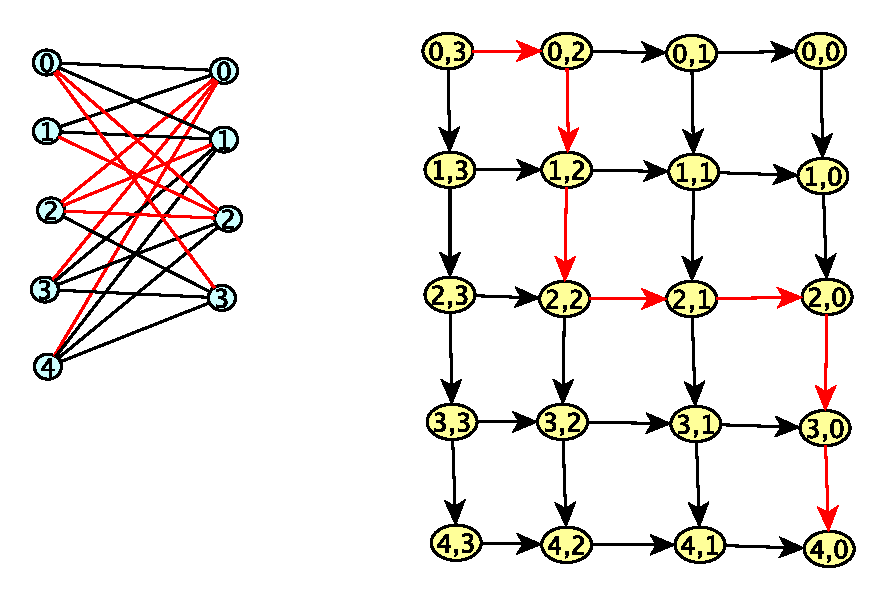
\includegraphics[height=7cm]{images_these/NonCrossingM.pdf}}
	\caption[Un chemin dans $H$ associé à un ensemble d'arêtes croisées dans G]{ Un chemin dans H associé à un ensemble d'arêtes croisées dans $G$.}
	\label{NonCrossingM}
\end{figure}

\begin{Lem}\label{lem_antcste}
	Pour tout plus long chemin $P$ dans $H$, la contrainte antagoniste engendrée par $P$ est valide pour $MILP_{SMEPC}$.
\end{Lem}
La démonstration de ce lemme se trouve en annexe à la section \ref{lem_antcste_section}.

\subsection{Polytope des correspondances non croisées}\label{NonCross}
Soit $Q$ le polytope défini par les contraintes (\ref{poly_me}).

\begin{subequations}\label{poly_me}
	\begin{align}
0 \leq U_{i,j} \leq 1,& \forall 0 \leq i \leq N-1, 0 \leq j \leq M &\label{positivite}\\
\sum_{(i, j) \in E(P)} U_{i,j} \leq 1,& \forall  P \in {\cal P}. &\label{antichaine}
\end{align}
\end{subequations}


{\it Une antichaine} $A$ de $(V(H),\preceq)$ est un sous-ensemble d'éléments de $V(H)$ incomparables par paires, c'est-à-dire que $A$ est l'ensemble de sommets de $V(H)$ de telle sorte que soit $(i_1,j_1)\npreceq (i_2,j_2)$ ou $(i_2,j_2)\npreceq (i_1,j_1)$ pour tout $(i_1,j_1)\in A, (i_2,j_2) \in A,(i_1,j_1)\neq (i_2,j_2)$.

Le polytope $Q$ est précisément le polytope de chaînes dont les sommets sont les vecteurs caractéristiques des antichaînes de $(V(H),\preceq)$.
%~(\cite{Sch}).

\begin{Lem}\label{lem_antichMatch}
	Une antichaine $A$ de $(V(H),\preceq)$ correspond à un ensemble de correspondance non croisée de $G$.
\end{Lem}
La démonstration de ce lemme se trouve en annexe à la section \ref{lem_antichMatch_section}.

D'après les lemmes (\ref{lem_antcste}) et (\ref{lem_antichMatch}), les sommets du polytope $Q$ sont des vecteurs caractéristiques des correspondances non croisés de $G$.

De plus, les contraintes antagonistes peuvent être utilisées pour renforcer la relaxation linéaire $RMILP_{SMEPC}$ de la section~\ref{sec4}.
Vérifier si une solution faisable $U$ de la relaxation linéaire satisfait des inégalités de type (\ref{clique_antag_P}) peut être effectué en temps polynomial
en cherchant le plus long chemin sur le digraphe acyclique $H$ avec l'algorithme de Bellman.

\subsection{Correspondance Time-consistent}

Cette section se concentre sur une sous-classe de correspondances non croisées.
Étant donné le graphe biparti complet $G=(I+J, E(G))$ et une fonction de poids $w : J \times J \rightarrow \mathbb{Z}_+$, nous disons que deux arêtes $(i,j)$ et $(i',j')$, avec $j <j'$, d'une correspondance dans $G$ sont \emph{ time-consistent} (respectivement \emph{ time-inconsistent}) si   $i+w(j,j') \leq i'$ (respectivement $i+w(j,j') > i'$). Un correspondance $C$ est dite {\it time-consistent} si $C$ est un sous-ensemble d'arêtes time-consistent par paires.

Notez que, comme $w(j, j') \geq 0, \textrm{ for all } 0 \leq j < j' \leq M$,  une correspondance time-consistent $C$ est aussi une correspondance non croisée de $G$. 
En effet, si deux arêtes $(i,j)$ et $(i',j')$ avec $j<j'$ appartiennent à $C$, alors nous avons $i' \geq i$, et les deux arêtes sont nécessairement non croisées.

Dans la tournée, le véhicule se déplace de la station $j$ vers une autre station $j'$ et ne peut pas atteindre $j'$ plus rapidement que le temps nécessaire pour le trajet en ligne droite entre $j$ et $j'$.
Les valeurs entières $w(j, j'), 0 \leq j < j' \leq M$, reflètent ce temps incompressible. 

\begin{Lem}\label{lem_ComplexIncons}
	Étant donné un graphe biparti complet $G=(I+J, E(G))$, une fonction de poids $w : J \times J \rightarrow \mathbb{Z}_+$ et un entier $k$, 
	le problème de la recherche d'une correspondance time-consistent de taille $k$ dans $G$ est $NP$-complet.
\end{Lem}
La démonstration de ce lemme se trouve en annexe à la section \ref{lem_ComplexIncons_section}.

Le lemme précédent suggère qu'une description complète du polytope des correspondances time-consistent est difficile à obtenir pour toute fonction de poids $w$. 
%%%%%%


\begin{figure}[H]
	\centerline{
		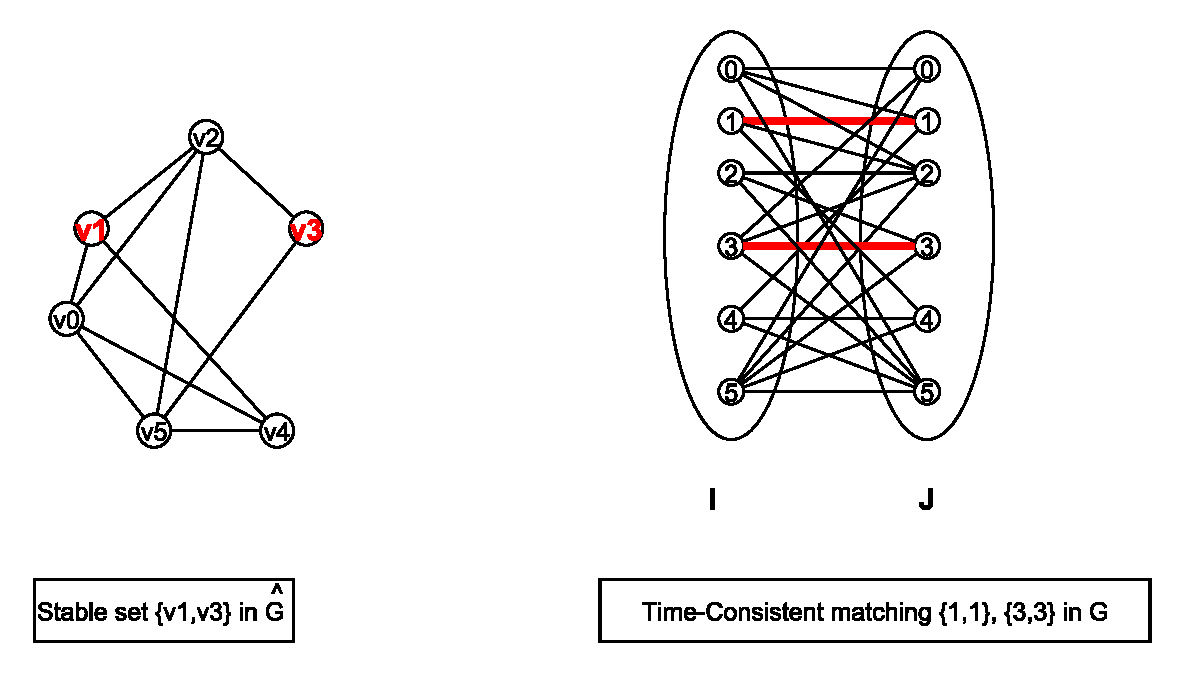
\includegraphics[height=7cm]{images_these/ConsistCompl.pdf}}
	\caption[Transformation d'un ensemble stable dans $H$ en un appariement conforme au temps dans G]{ Transformation d'un ensemble stable dans H en un croissement Time-consistent dans G.}
	\label{ConsistCompl}
\end{figure}

Dans la dernière partie de cette sous-section, nous supposons que la fonction de poids satisfait la propriété \emph{(SA)}.
$$ \begin{array}{lr}
\forall j_1, j_2, j_3 \in \llbracket 0, M \rrbracket, j_1 < j_2 < j_3 \Rightarrow w(j_1, j_2) + w(j_2, j_3) \leq w(j_1, j_3) & \textrm{(SA)}
\end{array} $$ 
%
Alors, si les paires $\{(i_1, j_1), (i_2, j_2) \}$ et  $\{(i_2, j_2), (i_3, j_3) \}$ sont time-inconsistent
pour certains $ 0\leq j_1 < j_2< j_3 \leq M$ et $ 0\leq i_1 < i_2 < i_3 \leq N-1$, alors 
la paire $\{(i_1, j_1), (i_3, j_3) \}$ est aussi time-inconsistent.

En ce qui concerne la propriété (SA), des contraintes valides peuvent être obtenues comme dans la section \ref{Non_crossing_matchings}.
Tout d'abord, complétons le graphe acyclique dirigé $H$ de la section \ref{Non_crossing_matchings} comme suit.
Pour tout $j < j'$ tel que $w(j, j') \geq 2$, nous ajoutons les arcs $((i' ,j'), (i,j))$ pour $ \max(0, i' - w(j, j') +1) \leq i \leq i'-1, 1 \leq i' \leq N-1$.
Désignons par $H_\textrm{tc}$ ce graphe modifié, par $A^+(H_\textrm{tc})$ l'ensemble des nouveaux arcs, et par ${\cal P}_\textrm{tc}$ l'ensemble des chemins $P$ qui commence à $(0, M)$ et se termine à $(N-1, 0)$ dans $H_\textrm{tc}$.

Ainsi, pour un plus long chemin $P \in {\cal P}_\textrm{tc}$, la contrainte (\ref{clique_timecons_P}) est appelé une contrainte {\it time-consistent} associée à $P$. 
\begin{eqnarray}
\sum_{(i, j) \in E(P)} U_{i,j} \le 1 &\label{clique_timecons_P}
\end{eqnarray}

\begin{Lem}\label{lem_arc_time}
	Soit $(i_0', j_0') $  et $(i_0, j_0) $ deux sommets de $H_\textrm{tc}$ tel que	$i_0' > i_0 $ et $j_0' > j_0 $. S'il existe un chemin dans $H_\textrm{tc}$ de $(i_0', j_0') $ à $(i_0, j_0) $, alors l'arc $((i_0', j_0'), (i_0, j_0)) $ existe dans $A^+(H_\textrm{tc})$.
\end{Lem}
La démonstration de ce lemme se trouve en annexe à la section \ref{dem_PTASlem_arc_time_section}.

\begin{Lem}\label{lem_timecons}
	Pour tout plus long chemin $P$ dans $H_\textrm{tc}$, la contrainte time-consistent induit par $P$ est valide pour $MILP_{SMEPC}$.
\end{Lem}
La démonstration de ce lemme se trouve en annexe à la section \ref{lem_timecons_section}.

De la même façon qu'à la section \ref{NonCross}, on peut voir que le polytope $Q_{t_c}$, défini par les inégalités (\ref{positivite}) et (\ref{clique_timecons_P}), pour tout chemin $P \in {\cal P}_\textrm{tc}$,
décrit la surface convexe des vecteurs qui caractérisent des correspondances time-consistent, lorsque la propriété $(SA)$ est satisfaite.

Pour $0\leq j<j'\leq M$, soit $\tilde{w}(j, j')=\sum_{k=j+1}^{j'-1} t_k, j'>j+1$ et $0$ sinon. 
il est évident que les valeurs $\tilde{w}(j,j')$ satisfont la propriété $(SA)$ et permettent une génération de contraintes time-consistent.
% ce qui est testé dans la partie expérimentale.


}
\section{Complexité du modèle SMEPC}
\label{NP-hard_SMEPC}
Dans cette partie,nous montrons que, même lorsque le coût fixe de production $Cost^F$ est nul, le \textbf{SMEPC} se réduit au problème du sac à dos. Cela nous permet d'établir le théorème \ref{smepc_difficilee}. 
\begin{theo}\label{smepc_difficilee}
SMEPC est NP-difficile.
\end{theo}
%\subsection{Généralités sur la complexité}
%définir les termes de compléxité
%\subsection{Démonstration : SMEPC est NP-difficile}
La démonstration de ce théorème se trouve en annexe à la section \ref{smepc_difficilee_section}.

 Après la présentation des résultats des expérimentations, nous nous attaquerons à la résolution proprement dites du problème à l'aide d'un schéma de programmation dynamique.  


\section{Expérimentations numériques}
\label{num_MIP}
\subsection{Objectifs et contexte technique}
L'objectif des expérimentations est de tester les formulations linéaires que nous avons proposé. Les modèles ont été implémentés en C++ et l'IDE utilisé est Visual Studio 2017.
Les expérimentations sont réalisées sur un ordinateur équipé d'un processeur AMD EPYC 7H12 64-Core, 512 Go de RAM et
fonctionnent sous Gnu/linux Ubuntu 20.04.2. Une première série d'expérimentations est réalisée au cours de laquelle CPLEX 12.10 est utilisé en mode 8 \textit{threads} 
%avec tous ses paramètres réglés sur leurs valeurs par défaut 
et le temps maximum du CPU est fixé à 3 heures. Les bornes supérieures obtenues seront utilisées comme valeurs de référence pour calculer les gaps tout au long de ce document. Une deuxième série d'expérimentations est réalisée au cours de laquelle CPLEX 12.10 est utilisé en mode \textit{single-threads} et le temps maximum du CPU est fixé à 1 heure.% avec tous ses paramètres réglés sur leurs valeurs par défaut 

\subsection{Procédés de génération d'instances du SMEPC}
\label{Gen_instance}
Pour faire des expérimentations, on a besoin d'instances du problème SMEPC. Étant donné que ce dernier est un nouveau problème, on a dû concevoir des procédés de génération de ses instances. On a un ensemble de 50 instances qui se subdivisent en deux paquets d'instances (paquet INST\_CTE et paquet INST\_VAR) car elles sont générées avec deux procédés différents. On a fixé que toutes nos entrées soient des valeurs entiers donc toutes nos variables le seront aussi. Dans cette section, on décrit les deux procédés de génération. 

Le paquet d'instances INST\_VAR a été généré avec une loi uniforme c'est pour cette raison que ces instances se \og ressemblent \fg{}. 
Pour pouvoir tester les performances de nos modèles on avait besoin d'instances suffisamment \og variées \fg{}, on a donc généré les instances du paquet INST\_CTE.
La génération d'instances ici consiste à générer le nombre de stations, les cordonnées de ces stations, les cordonnées du dépôt et les cordonnées de la micro-usine, le temps maximal, la durée d'une période, les rendements de production, les couts variables , les couts fixes de production, les quantités d'hydrogènes initiales dans le véhicule et dans la citerne et les capacités du véhicule et de la citerne.

Certaines étapes de la génération sont communes aux deux méthodes à l'instar de :
\begin{itemize}[label=$\square$]
	\item$xrectangle$, $yrectangle$ : Limite des coordonnées des stations respectivement sur l'axe des abscisses et l'axe des ordonnées. On considère que deux stations ne peuvent pas avoir les mêmes coordonnées. On fixe le rectangle dans lequel on place les stations aléatoirement, une station est un point dans le plan. Les valeurs entières $xrectangle$ et $yrectangle$ représentent respectivement la longueur en abscisse et en ordonné de ce rectangle (Voir figure \ref{Fr_gen_station}). Avec par exemple $(xrectangle,yrectangle) \in [1, M]^2 $. 
	\begin{figure}[H]
		\centerline{
			\includegraphics[height=8cm]{images_these/gen_station.pdf}}
		\caption[Plan contenant les stations]{Plan contenant les stations.}
		\label{Fr_gen_station}
	\end{figure}
	Si le dépôt a pour coordonnées $(a,b)$ alors la micro-usine aura pour coordonnées $(a,b+1)$ car on impose qu'il y ait une distance de 1 unité entre le dépôt et la micro-usine.
	
	%Nous fixons aléatoirement les stations comme des points dans un rectangle de dimension $xrectangle \times yrectangle$ , où deux stations ne peuvent pas avoir les mêmes coordonnées. Lamicro-usine sera proche du dépôt. Les coordonnées de la micro-usine sont $(x,y+1)$.
	\item A partir de ces coordonnées, la matrice des valeurs de distances est calculée comme la valeur arrondie de la distance euclidienne
	entre deux stations, et la matrice des valeurs d'énergie comme la valeur de la distance de Manhattan.
	Autrement dit, les valeurs de distances $d_j$, $d^*_j$, $t_j$ et les valeurs d'énergies $e_j$, $\varepsilon_j$, $\varepsilon^*_j$ correspondent respectivement à l'arrondi (partie entière supérieure) de la distance euclidienne et à la distance de Manhattan.
\end{itemize}
\subsubsection{Génération du paquet d'instances INST\_VAR}
On génère 30 instances avec le procédé de génération décrit par la suite.
 Nous fixons $M$ et $p$, et générons aléatoirement les stations $j$ et la station particulière $Depot$ comme point de l'espace $\mathbb{R}^2$.  
 On génère des instances aléatoirement de la façon suivante :

\begin{enumerate}
	\item On fixe aléatoirement $M$ le nombre de stations ($M>2$). Car on doit avoir au moins deux stations pour réaliser les tâches de transport et de livraison.
	\item On fixe aléatoirement $p$ la taille d'une période.
	\item On fixe le paramètre de la fonction objectif $\alpha=1$.% et $\beta=1$. 
	%\item On fixe le rectangle dans lequel on place les stations aléatoirement, une station est un point dans le plan. Les valeurs entières $xrectangle$ et $yrectangle$ représentent respectivement la longueur en abscisse et en ordonné de ce rectangle (Voir figure \ref{Fr_gen_station}). Avec par exemple $(xrectangle,yrectangle) \in [1, M]^2 $. 
%	\begin{figure}[H]
	%	\centerline{
	%		\includegraphics[height=8cm]{images_these/gen_station.pdf}}
	%	\caption[Plan contenant les stations]{Plan contenant les stations.}
	%	\label{Fr_gen_station}
	%\end{figure}
	%Si le dépôt a pour coordonné $(a,b)$ alors la micro-usine aura pour coordonnée $(a,b+1)$ car on impose qu'il y ait une distance de 1 unité entre le dépôt et la micro-usine.
	\item On fixe $E_0$, par exemple $E_0 \in [1, M]$. $E_0$ doit au moins être égale à 1 car il faut pouvoir se rendre à la micro-usine à partir du dépôt initial.
	\item On fixe le paramètre entier $param\_vmax$, par exemple $param\_vmax \in [2,3]$. On calcule $C^{Veh}$ tel que $C^{Veh}= \frac{\sum_{j \leq M} e_j }{ param\_vmax} +E_0$. L'idée ici est d'imposer qu'il faut au moins $param\_vmax$ recharges pour pouvoir finir la tournée.
	\item On fixe le paramètre entier $param\_cit \in [1,3]$. On calcule $C^{Tank}$ tel que $C^{Tank}=param\_cit \times C^{Veh}$. L'idée ici est d'imposer que si la citerne est pleine on peut remplir au plus $param\_cit$ fois le réservoir du véhicule sans production. 
	
	\item On fixe $Cost^F$, par exemple $Cost^F \in [1, 3\times M]$.  
	\item On fixe $H_0$, par exemple $H_0 \in [0, M]$. %On évite que $H_0$ soit très grand pour être certain qu'il y aura production.
	\item On fixe le paramètre entier $param\_tmax$, par exemple $param\_tmax\in [2,3]$. On calcule $TMax$ tel que $TMax \geq \sum_{j \leq M} d_j \times param\_tmax$. On fixe $TMax$ ainsi pour être sûr d'avoir suffisamment de temps pour finir la tournée.
	\item On calcule $N=\lceil \frac{TMax}{p}\rceil$.% en s'assurant que $N$ soit une valeur entière en prenant la partie entière supérieure.
	\item On fixe le paramètre entier $xrendement$, par exemple $xrendement \in [2,3]$. Le rendement de production de chaque période est fixé aléatoirement dans l'intervalle $[1, \frac{C^{Tank}}{xrendement}]$. L'idée ici est d'imposer qu'il faudrait au moins produire sur deux périodes pour pouvoir remplir la citerne.
	\item On fixe le paramètre entier $xcout$, par exemple $xcout \in [1, M]$. Le coût de production de chaque période est fixé aléatoirement dans l'intervalle $[1, xcout]$.
\end{enumerate}

%Pour contrôler la taille des instances, on s'assure que le nombre d'états générés maximal ne dépasse pas un certains seuil noté $SEUIL\_STATE$ (Avec la formule $C^{Veh}\times C^{Tank} \times  M\times N \times 2 \leq SEUIL\_STATE$).

%Ensuite, nous fixons $C^{Tank}$, $C^{Veh}$ et $TMax$, de telle sorte que cela assure l'existence d'une solution réalisable. Enfin, nous fixons les coefficients de coût, de telle sorte que le coût fixe $Cost^F$ soit au moins égal au plus grand coefficient $Cost^V_i$, $i = 0, \dots, N - 1$. 

%Dans le cas présent, nous utilisons un ensemble de 30 instances, avec les caractéristiques $N$, $M$, $TMax$, $p$, $C^{Veh}$, $C^{Tank}$ présenté par le tableau (\ref{tab:inst}). La signification de ces caractéristiques est :

%\begin{itemize}[label=$\square$]
%	\item $N$ : Nombre de périodes de production ; 
%	\item $M$ : Nombre de stations (Dépôt et micro-usine exclus) ; 
%	\item $TMax$ : Le délai maximal pour que le véhicule puisse effectuer sa tournée ;
%	\item $p$ : Durée en unités de temps d'une période de production ;
%	\item $C^{Veh}$ : Capacité du réservoir d'hydrogène du véhicule ; 
%	\item $C^{Tank}$ : Capacité de la citerne d'hydrogène.
%\end{itemize}

\subsubsection{Génération du paquet d'instances INST\_CTE}
On génère 20 instances avec le procédé de génération décrit par la suite. Avant de le décrire on présente les paramètres du processus de génération :
\begin{itemize}[label=$\square$]
	%\item $N$ : Nombre de périodes ;
	%\item $M$ : Nombre de stations, sans compter le Dépôt et la micro-usine ;
	%\item $xrectangle$, $yrectangle$ : Limite des coordonnées des stations respectivement sur l'axe des abscisses et l'axe des ordonnés ;
	\item $K $ : Le nombre d'intervalles, ainsi les N périodes seront divisées en $K$ intervalles. Pour des raisons de
	simplicité, nous allons faire en sorte que ces intervalles aient le même nombre de périodes. Nous ajoutons le paramètre $n$, qui sera le nombre de périodes d'un intervalle.
	Pour ce motif, $N$ ne sera pas un paramètre et il sera calculé comme $N= n\times K$.
	\item $Q$ exprime la contrainte induite par les besoins énergétiques (énergie à recharger) du véhicule et la capacité de stockage du véhicule, il s'agit du
	nombre de recharges prévu.
	\item $H$ : Le rapport entre la capacité de la citerne et le réservoir du véhicule.
	\item $R$ exprime la contrainte induite par les besoins énergétiques du véhicule sur l'activité de production.
	\item $S$ : Le rapport entre la part du coût due à la consommation d'énergie et la part
	du coût due à l'activation de la micro-usine.
	%\item $\alpha$ : Le taux de conversion qui permet de transformer le temps en valeur de coût. Ce paramètre seracalculé en multipliant un coefficient Cα par le coût unitaire moyen.
	
\end{itemize}


Nous calculons l'énergie minimale attendue $E^*$ comme l'énergie nécessaire dans une tournée simple construite de la
manière suivante : en partant du dépôt, nous sélectionnons itérativement la station non visitée la plus proche jusqu'à ce que toutes les stations soient visitées, puis, nous retournons au dépôt final. Nous calculons également l'énergie moyenne pour
se rendre à la micro-usine $E_{mean}^{MP}=\frac{1}{M+1}\sum_{ 0 \leq i \leq M}\varepsilon_i$.

Pour chaque intervalle $k \in K$, nous générons aléatoirement 2 nombres $\Pi_k$ avec $k \in 1, \dots, 5$ et $\Theta_k$ avec $k \in 1, \dots, 3$.
Pour chaque période $i$ de l'intervalle $k$, nous générons aléatoirement un taux de production $RAux_i$
et un coût de production variable $Cost^V_i$
selon la distribution uniforme respectivement à l'intérieur des intervalles $[\Pi_k/2, 3\Pi_k/2]$ et $[\Theta_k/2, 3\Theta_k/2]$.
Ensuite, nous obtenons le coût de production $R_i = \lambda\times RAux_i$,
en choisissant $\lambda$ de telle sorte que $\sum_i R_i=R\times E^*$. Nous calculons le coût moyen unitaire : $C_{mean}=(\sum_i Cost_i^V/R_i)\times N$. 

Nous fixons $C^{Veh} = E^*/Q + E^{MP}_{mean}$, nous ajoutons $E^{MP}_{mean}$ pour prendre en compte le fait que le véhicule
a également besoin de capacité pour aller se ravitailler en carburant et pour les bonnes tournées, le nombre de recharges est
approximativement $Q$. Nous fixons $C^{Tank} = H \times C^{Veh}$ et nous fixons le coût de production fixe : $Cost^F=\frac{C_{mean}\times E^*}{2S\times (1+E^*/C^{Veh})}$.

\subsection{Caractéristiques des instances}
Toutes les séries d'expériences concernent les instances présentées dans les tableaux (\ref{tab:inst}) et (\ref{tab:inst2}) avec les notations suivantes :

\begin{itemize}[label=$\square$]
	\item $num$ : Numéro de l'instance ;
	\item $M$ : Nombre de stations ;
	\item $N$ : Nombre de périodes ;
	\item $p$ : Durée d'une période ;
	\item $H_0$ : Quantité d'hydrogène initiale dans la citerne ;
	\item $C^{Tank}$ : Capacité maximale de la citerne ;
	\item $E_0$ : Quantité d'hydrogène initiale dans le réservoir du véhicule ;
	\item $C^{Veh}$ : Capacité maximale du réservoir ;
	\item $LTour$ : Durée de la tournée sans recharge ;
	\item $ETour$ : Énergie de la tournée sans recharge.
\end{itemize}
Les tableaux (\ref{tab:inst}) et (\ref{tab:inst2}) représentent respectivement les caractéristiques du paquet d'instances INST\_VAR et celles du paquet d'instances INST\_CTE.
On fait les remarques suivantes :
\begin{itemize}[label=$\square$]
	\item  Pour la plupart des instances du paquet INST\_VAR, l'énergie initial $E_0$ du véhicule est très petite par rapport à l'énergie de la tournée sans recharge $ETour$. Or cela n'est pas le cas pour les instances du paquet INST\_CTE ;
	\item Pour la plupart des instances du paquet INST\_VAR, l'énergie initial $E_0$ du véhicule est très petite par rapport à la capacité du véhicule $C^{Veh}$. Or cela n'est pas le cas pour les instances du paquet INST\_CTE ; on fait la même remarque pour $H_0$ par rapport à $C^{Tank}$ ;
	\item Les capacités du véhicule et de la citerne du paquet d'instances INST\_VAR sont très élevées par rapport à celles du paquet d'instances INST\_CTE ;
	\item Le nombre de périodes $N$ des instances du paquet INST\_CTE est constant, or, dans le paquet d'instances INST\_VAR on a différentes valeurs de $N$ ;
	\item Pour la plupart des instances, les valeurs de $N$ du paquet d'instances INST\_VAR sont très élevées par rapport à celles du paquet d'instances INST\_CTE ;
	\item Pour la plupart des instances, les valeurs de $p$ du paquet d'instances INST\_VAR sont très faibles par rapport à celles du paquet d'instances INST\_CTE.
\end{itemize}

\subsubsection{Caractéristiques des instances du paquet INST\_VAR}
%%%%%%Ar  DAM
Le tableau (\ref{tab:inst}) présente les caractéristiques des instances du paquet INST\_VAR.
Le paquet d'instances INST\_VAR est constitué de 30 instances. On a des instances de 8, 10, 12, 15, 20, 30, 50, 70 et 100 stations. La durée d'une période vaut 1, 2, 4, 5, 6, 8 et 10.
\begin{table}[H]
	\centering
	\small{
		\begin{tabular}{|r|r|r|r|r|r|r|r|r|r|}
			\hline
			\toprule
			\rowcolor{cyan}	\textbf{num} &$\mathbf{M}$ & $\mathbf{N}$ & $\mathbf{p}$ &  $\mathbf{H_0} $ & $\mathbf{C^{Tank}}$ & $\mathbf{E_0}$ & $\mathbf{C^{Veh}}$ & \textbf{LTour} & \textbf{Etour} \\
			\midrule
			\hline
			1	&	8	&	20	&	4	&	6	&	25	&	8	&	12	&	20	&	20	\\ \hline
			2	&	8	&	25	&	4	&	5	&	20	&	8	&	10	&	25	&	26	\\ \hline
			3	&	8	&	40	&	5	&	10	&	70	&	20	&	30	&	44	&	50	\\ \hline
			4	&	10	&	36	&	2	&	8	&	25	&	9	&	12	&	36	&	38	\\ \hline
			5	&	10	&	50	&	4	&	6	&	40	&	10	&	20	&	50	&	54	\\ \hline
			6	&	10	&	94	&	1	&	3	&	30	&	4	&	15	&	47	&	52	\\ \hline
			7	&	12	&	32	&	4	&	0	&	50	&	4	&	25	&	63	&	68	\\ \hline
			8	&	12	&	50	&	4	&	3	&	36	&	3	&	18	&	50	&	58	\\ \hline
			9	&	15	&	160	&	4	&	8	&	240	&	20	&	120	&	426	&	556	\\ \hline
			10	&	20	&	108	&	10	&	20	&	390	&	10	&	190	&	716	&	894	\\ \hline
			11	&	10	&	80	&	2	&	10	&	40	&	10	&	20	&	38	&	38	\\ \hline
			12	&	15	&	327	&	4	&	20	&	400	&	11	&	140	&	653	&	790	\\ \hline
			13	&	20	&	180	&	6	&	3	&	500	&	20	&	170	&	718	&	834	\\ \hline
			14	&	20	&	440	&	5	&	100	&	350	&	50	&	170	&	910	&	1164	\\ \hline
			15	&	30	&	177	&	8	&	6	&	420	&	10	&	200	&	944	&	1188	\\ \hline
			16	&	30	&	260	&	6	&	50	&	400	&	50	&	200	&	1034	&	1320	\\ \hline
			17	&	30	&	544	&	4	&	10	&	560	&	15	&	250	&	1088	&	1382	\\ \hline
			18	&	50	&	265	&	10	&	6	&	400	&	9	&	200	&	1764	&	2216	\\ \hline
			19	&	50	&	500	&	8	&	100	&	420	&	50	&	180	&	1565	&	2000	\\ \hline
			20	&	70	&	328	&	10	&	15	&	550	&	25	&	270	&	2183	&	2766	\\ \hline
			21	&	30	&	1100	&	2	&	100	&	400	&	80	&	200	&	1097	&	1342	\\ \hline
			22	&	30	&	1200	&	2	&	100	&	400	&	70	&	200	&	957	&	1200	\\ \hline
			23	&	50	&	634	&	6	&	50	&	300	&	50	&	150	&	1542	&	1938	\\ \hline
			24	&	50	&	850	&	4	&	20	&	400	&	50	&	180	&	1941	&	2500	\\ \hline
			25	&	50	&	1125	&	4	&	20	&	700	&	50	&	280	&	1718	&	2128	\\ \hline
			26	&	70	&	383	&	8	&	20	&	760	&	15	&	240	&	2039	&	2590	\\ \hline
			27	&	70	&	683	&	8	&	8	&	850	&	14	&	370	&	2185	&	2826	\\ \hline
			28	&	70	&	984	&	6	&	50	&	750	&	40	&	250	&	2340	&	2926	\\ \hline
			29	&	100	&	651	&	8	&	100	&	600	&	60	&	200	&	3471	&	4360	\\ \hline
			30	&	100	&	800	&	10	&	100	&	950	&	100	&	430	&	3095	&	3796	\\ \hline
			
			\bottomrule
		\end{tabular}%
	}\caption{Caractéristiques des instances du paquet INST\_VAR}
	\label{tab:inst}%
\end{table}%
\subsubsection{Caractéristiques des instances du paquet INST\_CTE}
Le tableau (\ref{tab:inst2}) présente les caractéristiques des instances du paquet INST\_CTE.
Le paquet d'instances INST\_CTE est constitué de 20 instances. On a des instances de 10, 20, 30, 50, 75 et 100 stations. Le nombre de périodes est fixe. Le nombre de périodes est 20 pour toutes les instances. La durée d'une période vaut 5, 10, 14, 34, 58 et 65.  
\begin{table}[H]
	\centering
	\small{
		\begin{tabular}{|r|r|r|r|r|r|r|r|r|r|}
			\hline
			\toprule
			\rowcolor{cyan}	\textbf{num} &$\mathbf{M}$ & $\mathbf{N}$ & $\mathbf{p}$ &  $\mathbf{H_0} $ & $\mathbf{C^{Tank}}$ & $\mathbf{E_0}$ & $\mathbf{C^{Veh}}$ & \textbf{LTour} & \textbf{Etour} \\
			\midrule
			\hline
			31	&	10	&	20	&	5	&	51	&	73	&	34	&	49	&	48	&	54	\\ \hline
			32	&	10	&	20	&	5	&	48	&	69	&	32	&	46	&	50	&	56	\\ \hline
			33	&	10	&	20	&	5	&	42	&	60	&	28	&	40	&	47	&	54	\\ \hline
			34	&	10	&	20	&	5	&	54	&	78	&	36	&	52	&	46	&	52	\\ \hline
			35	&	20	&	20	&	10	&	65	&	94	&	32	&	47	&	84	&	100	\\ \hline
			36	&	20	&	20	&	10	&	72	&	104	&	36	&	52	&	73	&	78	\\ \hline
			37	&	20	&	20	&	10	&	42	&	60	&	42	&	60	&	78	&	82	\\ \hline
			38	&	20	&	20	&	10	&	35	&	51	&	35	&	51	&	101	&	112	\\ \hline
			39	&	20	&	20	&	10	&	34	&	49	&	34	&	49	&	73	&	80	\\ \hline
			40	&	30	&	20	&	14	&	85	&	122	&	85	&	122	&	136	&	156	\\ \hline
			41	&	50	&	20	&	34	&	65	&	93	&	43	&	62	&	218	&	238	\\ \hline
			42	&	50	&	20	&	34	&	56	&	81	&	37	&	54	&	205	&	224	\\ \hline
			43	&	75	&	20	&	58	&	102	&	147	&	41	&	59	&	275	&	308	\\ \hline
			44	&	75	&	20	&	58	&	109	&	157	&	44	&	63	&	217	&	232	\\ \hline
			45	&	100	&	20	&	65	&	198	&	284	&	49	&	71	&	265	&	278	\\ \hline
			46	&	100	&	20	&	65	&	232	&	332	&	58	&	83	&	283	&	298	\\ \hline
			47	&	100	&	20	&	65	&	233	&	333	&	77	&	111	&	274	&	284	\\ \hline
			48	&	100	&	20	&	65	&	256	&	366	&	85	&	122	&	386	&	424	\\ \hline
			49	&	100	&	20	&	65	&	203	&	291	&	67	&	97	&	253	&	260	\\ \hline
			50	&	100	&	20	&	65	&	165	&	237	&	55	&	79	&	256	&	268	\\ \hline
			
			\bottomrule
		\end{tabular}%
	}\caption{Caractéristiques des instances du paquet INST\_CTE}
	\label{tab:inst2}%
\end{table}%


\subsection{Caractéristiques des solutions}
Dans cette section, on présente les caractéristiques des solutions des 50 instances générées. Ces solutions ont été obtenues par le modèle $MILP_{SMEPC}$ en y ajoutant les contraintes (STC), (EC1), (EC2) et (EC3). Lorsque la solution optimale n'est pas connue, on donne les caractéristiques de la borne supérieure. La liste de ces caractéristiques est :
\begin{itemize}[label=$\square$]
	\item $\mathbf{nbRech}$ : Nombre de recharges ;
	\item $\mathbf{nbSetup}$ : Nombre d'activations de la micro-usine
	\item $\mathbf{prod}$ : Hydrogène produite pour réaliser la tournée ;
	\item  $\mathbf{conso} $ :  Hydrogène consommée par le véhicule pour réaliser la tournée ;
	\item $\mathbf{wait time}$ : Temps d'attente du véhicule ;
	\item $\mathbf{cost time}$ : Coût en temps de la solution ;
	 \item $\mathbf{cost prod}$ : Coût de production de la solution.
\end{itemize}

En moyenne, on constate que pour toutes les instances, la durée de la tournée $\mathbf{cost time}$ est très élevée par rapport à la durée de la tournée sans recharge  $LTour$, ce qui peut vouloir dire que le véhicule attend \og beaucoup \fg{} avant de se recharger ou que la durée des détours est très élevée. On remarque aussi qu'il n'y a pas un grand gap entre la quantité d'hydrogène produite et la quantité d'hydrogène consommée, ce qui peut vouloir dire qu'on ne produit pas de façon excessive.

Les tableaux (\ref{tab:sol}) et (\ref{tab:sol2}) représentent respectivement les caractéristiques des solutions du paquet d'instances INST\_VAR et celles du paquet d'instances INST\_CTE.
On fait les remarques suivantes :
\begin{itemize}[label=$\square$]
	\item Concernant les instances du paquet INST\_VAR, le temps d'attente $wait time$ du véhicule est très faible par rapport au coût en temps $cost time$ du processus, on passe en moyenne 58,62\% du temps à attendre. Or cela n'est pas la cas pour les instances du paquet INST\_CTE ;
	\item Globalement, le nombre de recharge du paquet d'instances INST\_VAR est supérieur au nombre de recharge du paquet d'instances INST\_CTE, cela est peut-être dû au fait que les valeurs $E_0$ du paquet INST\_VAR sont très petites par rapport aux valeurs $Etour$ ;
	\item  Concernant les instances du paquet INST\_VAR, le coût de production $cost prod$ est très faible par rapport au coût en temps $cost time$. Or cela n'est pas le cas pour les instances du paquet INST\_CTE. 
	\item La quantité d'hydrogène produite et consommée du paquet d'instances INST\_VAR est très élevée par rapport à celle du paquet d'instances INST\_CTE ; 
\end{itemize}
\subsubsection{Caractéristiques des solutions des instances du paquet INST\_VAR}
Le tableau (\ref{tab:sol}) présente les caractéristiques des solutions des instances du paquet INST\_VAR. 

 %Les instances 24, 25, 29 et 30 sont celles dont on n'a pas pu obtenir les solutions en moins d'une heure, on les a laissé s'exécuter durant plus longtemps. Pour avoir une borne supérieure, on a dû mettre le temps limite à 3 heures en utilisant 8 threads. %Pour obtenir les solutions de ces quatre instances on a supprimé du modèle $MILP_{SMEPC}$ les contraintes symétriques (\ref{39}).

 % En moyenne, la durée de la tournée $\mathbf{cost time}$ est très élevée par rapport à la durée de la tournée sans recharge  $LTour$, ce qui peut vouloir dire que le véhicule attend \og beaucoup \fg{} avant de se recharger ou que la durée des détours est très élevée. On remarque aussi qu'il n'y a pas un grand gap entre la quantité d'hydrogène produite et la quantité d'hydrogène consommée, ce qui peut vouloir dire qu'on ne produit pas de façon excessive.

\begin{table}[H]
	\centering
	\small{
		\begin{tabular}{|r|r|r|r|r|r|r|r|}
			\hline
			\toprule
			\rowcolor{cyan}	\textbf{num} &$\mathbf{nbRech}$ & $\mathbf{nbSetup}$ & $\mathbf{prod}$ &  $\mathbf{conso} $ & $\mathbf{wait time}$ & $\mathbf{cost time}$ & $\mathbf{cost prod}$  \\
			\midrule
			\hline
			1	&	3	&	2	&	29	&	28	&	30	&	57	&	74	\\ \hline
			2	&	5	&	2	&	34	&	34	&	40	&	73	&	78	\\ \hline
			3	&	3	&	2	&	64	&	62	&	25	&	81	&	63	\\ \hline
			4	&	5	&	2	&	42	&	42	&	26	&	67	&	73	\\ \hline
			5	&	5	&	2	&	63	&	60	&	29	&	85	&	76	\\ \hline
			6	&	7	&	4	&	72	&	72	&	8	&	73	&	105	\\ \hline
			7	&	5	&	3	&	92	&	90	&	39	&	121	&	101	\\ \hline
			8	&	6	&	2	&	69	&	66	&	58	&	121	&	71	\\ \hline
			9	&	7	&	4	&	624	&	622	&	40	&	509	&	135	\\ \hline
			10	&	8	&	4	&	1104	&	1084	&	133	&	1001	&	138	\\ \hline
			11	&	4	&	2	&	61	&	58	&	17	&	75	&	59	\\ \hline
			12	&	10	&	3	&	952	&	946	&	67	&	819	&	93	\\ \hline
			13	&	7	&	3	&	975	&	972	&	70	&	867	&	89	\\ \hline
			14	&	12	&	5	&	1442	&	1412	&	89	&	1231	&	141	\\ \hline
			15	&	8	&	5	&	1354	&	1328	&	107	&	1196	&	150	\\ \hline
			16	&	9	&	4	&	1391	&	1390	&	76	&	1160	&	131	\\ \hline
			17	&	8	&	3	&	1474	&	1424	&	50	&	1182	&	103	\\ \hline
			18	&	15	&	8	&	2400	&	2400	&	215	&	2125	&	248	\\ \hline
			19	&	17	&	6	&	2211	&	2210	&	187	&	1977	&	236	\\ \hline
			20	&	13	&	7	&	2851	&	2848	&	207	&	2449	&	210	\\ \hline
			21	&	11	&	5	&	1545	&	1488	&	28	&	1279	&	131	\\ \hline
			22	&	11	&	4	&	1500	&	1456	&	27	&	1221	&	121	\\ \hline
			23	&	22	&	11	&	2510	&	2510	&	178	&	2276	&	314	\\ \hline
			24	&	22	&	11	&	3036	&	3022	&	111	&	2517	&	288	\\ \hline
			25	&	12	&	5	&	2293	&	2278	&	65	&	1924	&	129	\\ \hline
			26	&	15	&	5	&	2617	&	2610	&	155	&	2244	&	112	\\ \hline
			27	&	11	&	5	&	2833	&	2828	&	113	&	2317	&	151	\\ \hline
			28	&	18	&	6	&	3374	&	3360	&	164	&	2879	&	175	\\ \hline
			29	&	30	&	10	&	4626	&	4616	&	411	&	4129	&	308	\\ \hline
			30	&	12	&	6	&	3871	&	3864	&	196	&	3362	&	160	\\ \hline
			
			
			\bottomrule
		\end{tabular}%
	}\caption{Caractéristiques des solutions des instances du paquet INST\_VAR}
	\label{tab:sol}%
\end{table}%
\subsubsection{Caractéristiques des solutions des instances du paquet INST\_CTE}
Le tableau (\ref{tab:sol2}) présente les caractéristiques des solutions des instances du paquet INST\_CTE. %En moyenne, on constate que la durée de la tournée $\mathbf{cost time}$ est très élevée par rapport à la durée de la tournée sans recharge  $LTour$, ce qui peut vouloir dire que le véhicule attend \og beaucoup \fg{} avant de se recharger ou que la durée des détours est très élevée. On remarque aussi qu'il n'y a pas un grand gap entre la quantité d'hydrogène produite et la quantité d'hydrogène consommée, ce qui peut vouloir dire qu'on ne produit pas de façon excessive.
\begin{table}[H]
	\centering
	\small{
		\begin{tabular}{|r|r|r|r|r|r|r|r|}
			\hline
			\toprule
			\rowcolor{cyan}	\textbf{num} &$\mathbf{nbRech}$ & $\mathbf{nbSetup}$ & $\mathbf{prod}$ &  $\mathbf{conso} $ & $\mathbf{wait time}$ & $\mathbf{cost time}$ & $\mathbf{cost prod}$  \\
			\midrule
			\hline
			31	&	2	&	2	&	59	&	56	&	16	&	66	&	175	\\ \hline
			32	&	3	&	2	&	64	&	64	&	23	&	81	&	277	\\ \hline
			33	&	2	&	2	&	56	&	56	&	11	&	61	&	162	\\ \hline
			34	&	2	&	2	&	54	&	54	&	11	&	61	&	141	\\ \hline
			35	&	4	&	2	&	121	&	114	&	53	&	151	&	106	\\ \hline
			36	&	3	&	1	&	98	&	92	&	57	&	141	&	85	\\ \hline
			37	&	2	&	2	&	87	&	84	&	32	&	111	&	66	\\ \hline
			38	&	4	&	4	&	122	&	120	&	62	&	171	&	111	\\ \hline
			39	&	4	&	4	&	118	&	114	&	47	&	151	&	162	\\ \hline
			40	&	2	&	4	&	169	&	160	&	38	&	177	&	159	\\ \hline
			41	&	6	&	6	&	290	&	290	&	355	&	613	&	288	\\ \hline
			42	&	7	&	6	&	283	&	280	&	363	&	613	&	827	\\ \hline
			43	&	9	&	8	&	464	&	402	&	743	&	1103	&	433	\\ \hline
			44	&	6	&	3	&	294	&	294	&	485	&	755	&	164	\\ \hline
			45	&	6	&	6	&	385	&	380	&	453	&	794	&	135	\\ \hline
			46	&	5	&	3	&	338	&	338	&	466	&	781	&	70	\\ \hline
			47	&	4	&	3	&	409	&	358	&	379	&	716	&	226	\\ \hline
			48	&	5	&	3	&	517	&	502	&	598	&	1041	&	209	\\ \hline
			49	&	4	&	3	&	340	&	340	&	394	&	716	&	115	\\ \hline
			50	&	6	&	6	&	385	&	372	&	503	&	846	&	234	\\ \hline
			
			
			
			\bottomrule
		\end{tabular}%
	}\caption{Caractéristiques des solutions des instances du paquet INST\_CTE}
	\label{tab:sol2}%
\end{table}%

\subsection{Résultats du modèle $MILP_{SMEPC}$ avec temps limite de 3 heures et 8 \textit{threads}}
Cette section présente les résultats du modèle $MILP_{SMEPC}$ avec les contraintes (STC), (EC1), (EC2) et (EC3) . %Les valeurs $BSup$ seront utilisées comme valeurs de références pour calculer les gaps dans tout ce document.
 Pour chaque instance, on donne la borne inférieure qu'on nomme $BInf$, la borne supérieure qu'on nomme $BSup$ et le temps CPU en secondes obtenue par CPLEX. \textbf{Ces valeurs $BSup$ seront utilisées comme valeurs de références pour calculer les gaps dans tout ce document}. $gapMI$ est le gap entre la borne inférieure et la borne supérieure % fixe le temps limite d'exécution à une heure. On ne présente ici que les résultats du meilleur modèle, c'est-à-dire celui ayant donné le plus de valeurs optimales en moins d'une heure. 
Des essais préliminaires ont été effectués avec la formulation de base de la section \ref{SMEPC_model} uniquement.  Sa faiblesse est rapidement apparue puisque CPLEX n'a pas pu trouver une solution réalisable à la majorité des instances après une heure de temps CPU. Nous observons alors qu'avec les contraintes \textit{Simple Time Constraints} (\ref{STC_1})	et (\ref{STC_2}), CPLEX peut atteindre une solution réalisable sur plus de la moitié de ces instances. Ceci explique pourquoi la formulation de référence $MILP_{SMEPC}$ intégrera les contraintes (STC).
Dans le cadre de la résolution en nombres entiers du modèle de référence, les tableaux (\ref{tab:resultSYM_STC}) et (\ref{tab:resultSYM_STC2}) montrent que 38 instances sur les 50 testées sont résolues de manière optimale. %Ces ensembles de données peuvent être considérés comme des instances {\it faciles }.
On fait les remarques suivantes :
\begin{itemize}[label=$\square$]
	
	\item On trouve la solution optimale de toutes les instances du paquet INST\_CTE, or on trouve la solution optimale de 18 instances du paquet INST\_VAR mais pour les 12 instances restantes on obtient moins de 5\% de gap entre $BSup$ et $BInf$ ;
	\item En moyenne, L'exécution des instances INST\_CTE est beaucoup plus rapide que celle de INST\_VAR.
\end{itemize}
\subsubsection{Résultats du modèle $MILP_{SMEPC}$ pour les instances du paquet INST\_VAR}
Le tableau (\ref{tab:resultSYM_STC}) présente les résultats du modèle $MILP_{SMEPC}$ avec les contraintes (STC), (EC1), (EC2) et (EC3) pour les instances du paquet INST\_VAR.
Concernant les 30 instances du paquet INST\_VAR, le modèle $MILP_{SMEPC}$ fournit la solution optimale de 18 instances en moins de 3 heures sur \textbf{8 \textit{threads}}.% Les ces instances 24, 25, 29 et 30 sont celles dont on n'a pas pu obtenir les solutions en moins d'une heure, on les a laissé s'exécuter durant plus longtemps. Pour avoir une borne supérieure, on a dû mettre le temps limite à 3 heures en utilisant 8 threads.
\begin{table}[H]
	\centering
	\small{
		\begin{tabular}{|r|r|r|r|r|}
			\hline
			\toprule
			\rowcolor{cyan}	\textbf{num} &$\mathbf{BInf}$ & $\mathbf{BSup}$ & $\mathbf{CPU}$ &$\mathbf{gapMI}$  \\
			\midrule
			\hline
		1	&	131	&	131	&	0,31	&	0,00	\\ \hline
		2	&	151	&	151	&	2,22	&	0,00	\\ \hline
		3	&	144	&	144	&	1,91	&	0,00	\\ \hline
		4	&	140	&	140	&	2,51	&	0,00	\\ \hline
		5	&	161	&	161	&	1,87	&	0,00	\\ \hline
		6	&	178	&	178	&	7,09	&	0,00	\\ \hline
		7	&	222	&	222	&	0,77	&	0,00	\\ \hline
		8	&	192	&	192	&	9,94	&	0,00	\\ \hline
		9	&	644	&	644	&	3,05	&	0,00	\\ \hline
		10	&	1139	&	1139	&	4,55	&	0,00	\\ \hline
		11	&	134	&	134	&	2,16	&	0,00	\\ \hline
		12	&	912	&	912	&	43,36	&	0,00	\\ \hline
		13	&	956	&	956	&	3,04	&	0,00	\\ \hline
		14	&	1372	&	1372	&	39,92	&	0,00	\\ \hline
		15	&	1346	&	1346	&	48,54	&	0,00	\\ \hline
		16	&	1291	&	1291	&	179,01	&	0,00	\\ \hline
		17	&	1285	&	1285	&	763,64	&	0,00	\\ \hline
		18	&	2372,45	&	2373	&	6708,77	&	0,02	\\ \hline
		19	&	2190,02	&	2213	&	10802,20	&	1,04	\\ \hline
		20	&	2562,58	&	2659	&	10802,40	&	3,63	\\ \hline
		21	&	1393,95	&	1410	&	10806,10	&	1,14	\\ \hline
		22	&	1334,71	&	1342	&	10804,70	&	0,54	\\ \hline
		23	&	2556,17	&	2590	&	10803,40	&	1,31	\\ \hline
		24	&	2763,18	&	2805	&	10804,00	&	1,49	\\ \hline
		25	&	2053	&	2053	&	1165,38	&	0,00	\\ \hline
		26	&	2343,35	&	2356	&	10805,60	&	0,54	\\ \hline
		27	&	2449,41	&	2468	&	10803,10	&	0,75	\\ \hline
		28	&	2944,06	&	3054	&	10803,90	&	3,60	\\ \hline
		29	&	4246,45	&	4437	&	10803,10	&	4,29	\\ \hline
		30	&	3410,42	&	3522	&	10803,60	&	3,17	\\ \hline
			
	\bottomrule
\end{tabular}%
}\caption[Résultats de $MILP_{SMEPC}$ sur INST\_VAR. Le temps limite est 3 heures sur 8 \textit{threads}]{Résultats du modèle $MILP_{SMEPC}$ sur les instances du paquet INST\_VAR. Le temps limite est 3 heures sur 8 \textit{threads}.}
\label{tab:resultSYM_STC}%
\end{table}%
\subsubsection{Résultats du modèle $MILP_{SMEPC}$ pour les instances du paquet INST\_CTE}
Le tableau (\ref{tab:resultSYM_STC2}) présente les résultats du modèle $MILP_{SMEPC}$ avec les contraintes (STC), (EC1), (EC2) et (EC3) pour les instances du paquet INST\_CTE. On obtient les solutions optimales des 20 instances du paquet INST\_CTE avec le modèle $MILP_{SMEPC}$ en moins de 3 heures sur \textbf{8 \textit{threads}}.
\begin{table}[H]
	\centering
	\small{
		\begin{tabular}{|r|r|r|r|}
			\hline
			\toprule
			\rowcolor{cyan}	\textbf{num} &$\mathbf{BInf}$ & $\mathbf{BSup}$ & $\mathbf{CPU}$   \\
			\midrule
			\hline
			31	&	241	&	241	&	0,414	\\ \hline
			32	&	358	&	358	&	0,443	\\ \hline
			33	&	223	&	223	&	0,163	\\ \hline
			34	&	202	&	202	&	0,266	\\ \hline
			35	&	257	&	257	&	0,66	\\ \hline
			36	&	226	&	226	&	0,614	\\ \hline
			37	&	177	&	177	&	0,643	\\ \hline
			38	&	282	&	282	&	0,602	\\ \hline
			39	&	313	&	313	&	1,62	\\ \hline
			40	&	336	&	336	&	1,197	\\ \hline
			41	&	901	&	901	&	9,169	\\ \hline
			42	&	1440	&	1440	&	3,091	\\ \hline
			43	&	1536	&	1536	&	29,316	\\ \hline
			44	&	919	&	919	&	13,367	\\ \hline
			45	&	929	&	929	&	50,343	\\ \hline
			46	&	851	&	851	&	21,56	\\ \hline
			47	&	942	&	942	&	10,719	\\ \hline
			48	&	1250	&	1250	&	27,978	\\ \hline
			49	&	831	&	831	&	53,674	\\ \hline
			50	&	1080	&	1080	&	39,143	\\ \hline
			
			
			\bottomrule
		\end{tabular}%
	}\caption[Résultats de $MILP_{SMEPC}$ sur INST\_CTE. Le temps limite est 3 heures sur 8 \textit{threads}]{Résultats du modèle $MILP_{SMEPC}$ sur les instances du paquet INST\_CTE. Le temps limite est 3 heures sur 8 \textit{threads}.}
	\label{tab:resultSYM_STC2}%
\end{table}%

\subsection{Résultats des modèles $RMILP_{SMEPC}$ et $MILP_{SMEPC}$ avec comme temps limite 1 heure sur 1 thread}
Nous présentons ici les résultats de tous les modèles sur les instances des paquets INST\_CTE et INST\_VAR.  Pour les résultats suivant, CPLEX 12.10 est utilisé en mode \textit{single-threads}. 
%avec tous ses paramètres réglés sur leurs valeurs par défaut.
 Le temps maximum du CPU est fixé à 1 heure.


 %On ne présente pas les résultats sur les instances du paquets INST\_CTE car ils aboutissent aux mêmes conclusions.
\subsubsection{Résultats du \textit{$RMILP_{SMEPC}$} avec comme temps limite 1 heure sur 1 thread }

Dans cette section, les expérimentations concernent la relaxation linéaire \textit{$RMILP_{SMEPC}$}. Nous étudions la contribution des inégalités données dans la section \ref{sec4}. Dans chaque cas, on donne la valeur optimale de la fonction objectif, le temps CPU et le gap à la solution optimale si elle existe ou à la meilleure borne, sinon.  Les tableaux (\ref{tab:frac1}), (\ref{tab:frac2}), (\ref{tab:frac3}) et (\ref{tab:frac4}) présentent les résultats pour :
\begin{itemize}[label=$\square$]
	\item (LR) : \textit{$RMILP_{SMEPC}$} la relaxation linéaire seule ;
	\item (LR)+(STC) : \textit{$RMILP_{SMEPC}$} lorsque seules les contraintes (STC) sont ajoutées ;
	\item (EC1+EC2) : \textit{$RMILP_{SMEPC}$} lorsque les contraintes (EC1) et (EC2) sont ajoutées à (LR)+(STC) ; 
	\item (EC3) : \textit{$RMILP_{SMEPC}$} lorsque les contraintes (EC3) sont ajoutées à (LR)+(STC) ;
	\item All energy : \textit{$RMILP_{SMEPC}$} lorsque les contraintes (EC1), (EC2) et (EC3)  sont ajoutées à (LR)+(STC).
\end{itemize}
Pour chaque instance, les résultats suivants sont spécifiés :
\begin{itemize}[label=$\square$]
	\item $CPU$ : Temps total du CPU en secondes ;
	\item $Obj$ : Valeur optimale du programme linéaire ;
	\item $GapF =  100 \times \frac{opt-Obj}{opt}$ : Pourcentage de l'erreur relative entre la meilleure solution réalisable $opt$ (C'est la solution optimale si l'instance a été résolu jusqu'à l'optimalité. Si une instance n'a pas été résolue jusqu'à l'optimalité, $opt$ est la borne supérieure de l'exécution de \textit{$MILP_{SMEPC}$} sur 8 \textit{threads} avec un temps limite de 3 heures (voir tableau (\ref{tab:resultSYM_STC}) et (\ref{tab:resultSYM_STC2})).) et la valeur optimale de la fonction objectif de la relaxation linéaire $Obj$. Les instances indiquées par "-" sont celles dont le temps de calcul de la solution optimale a dépassé 1h.
\end{itemize}
Les tableaux (\ref{tab:frac1}) et (\ref{tab:frac2}) présentent les résultats de la relaxation linéaire \textit{$RMILP_{SMEPC}$} du  paquet d'instances INST\_VAR.
Pareillement, les tableaux (\ref{tab:frac3}) et (\ref{tab:frac4}) présentent les résultats de la relaxation linéaire \textit{$RMILP_{SMEPC}$} du  paquet d'instances INST\_CTE. On constate que les contraintes (STC) sont les plus efficaces car ce sont elles qui améliore le plus le gap surtout sur les grandes instances. Mais elles induisent une légère augmentation du temps CPU. De plus, Les contraintes (EC) ont en général sur toutes les instances un faible impact sur la gap.
On fait les remarques suivantes :
\begin{itemize}[label=$\square$]

	\item L'ajout de la contrainte (STC) pour les instances du paquet INST\_VAR induit un plus grand écart que pour le paquet INST\_CTE parce que comme on l'a dit précédemment les solutions des instances INST\_VAR ont un coût temps très grand par rapport au coût production. C'est pour cette raison que l'amélioration de la partie temps a une grande incidence sur le coût final ;
	\item Les solutions obtenues pas ces modèles sur le paquet d'instances INST\_VAR sont meilleures que celles obtenues sur les instances INST\_CTE. Donc ces modèles marchent mieux sur les instances INST\_VAR ;
	\item Le temps de calcul du paquet d'instances INST\_VAR est supérieur au temps de calcul des instances INST\_CTE.

\end{itemize}

%%%%%%%%%%%%%%%%%%%%%%%%%%%%%%%%%%%%%%%%%%%%%%%%
\begin{table}[H]
	\centering
	\small
	\begin{tabular}{|r|rrr|rrr|}
		\hline
		\toprule
		\rowcolor{cyan}	\multicolumn{4}{c}{\textbf{LR}}              & \multicolumn{3}{c}{\textbf{LR + STC}} \\ \hline
		\midrule
		\rowcolor{cyan}	\textbf{num} & \textbf{Obj} & \textbf{CPU} & \textbf{GapF} & \multicolumn{1}{r}{ \textbf{Obj}} & \textbf{CPU} & \textbf{GapF} \\ \hline
		\midrule
	1	&	44,15	&	0,0	&	66,29	&	68,18	&	0,0	&	47,95	\\ \hline
	2	&	36,94	&	0,0	&	75,53	&	64,89	&	0,1	&	57,02	\\ \hline
	3	&	30,93	&	0,1	&	78,52	&	79,51	&	0,1	&	44,79	\\ \hline
	4	&	45,34	&	0,0	&	67,62	&	82,52	&	0,0	&	41,06	\\ \hline
	5	&	46,42	&	0,1	&	71,17	&	97,27	&	0,0	&	39,58	\\ \hline
	6	&	41,26	&	0,1	&	76,82	&	97,79	&	0,1	&	45,06	\\ \hline
	7	&	52,00	&	0,1	&	76,57	&	124,84	&	0,0	&	43,77	\\ \hline
	8	&	39,97	&	0,0	&	79,18	&	96,43	&	0,0	&	49,78	\\ \hline
	9	&	80,16	&	0,1	&	87,55	&	523,61	&	0,1	&	18,69	\\ \hline
	10	&	59,41	&	0,1	&	94,78	&	883,52	&	0,1	&	22,43	\\ \hline
	11	&	27,60	&	0,1	&	79,40	&	78,80	&	0,0	&	41,19	\\ \hline
	12	&	37,90	&	0,2	&	95,84	&	717,05	&	0,4	&	21,38	\\ \hline
	13	&	33,34	&	0,1	&	96,51	&	794,71	&	0,2	&	16,87	\\ \hline
	14	&	69,60	&	0,4	&	94,93	&	1049,27	&	1,3	&	23,52	\\ \hline
	15	&	68,84	&	0,2	&	94,89	&	1114,54	&	0,3	&	17,20	\\ \hline
	16	&	62,16	&	0,3	&	95,19	&	1120,57	&	0,4	&	13,20	\\ \hline
	17	&	49,10	&	0,5	&	96,18	&	1155,17	&	2,4	&	10,10	\\ \hline
	18	&	125,35	&	0,6	&	94,72	&	1942,44	&	0,8	&	18,14	\\ \hline
	19	&	137,60	&	1,4	&	93,78	&	1826,41	&	5,0	&	17,47	\\ \hline
	20	&	106,04	&	1,0	&	96,01	&	2311,54	&	1,5	&	13,07	\\ \hline
	21	&	70,42	&	3,3	&	95,01	&	1240,39	&	10,6	&	12,03	\\ \hline
	22	&	60,27	&	2,7	&	95,51	&	1106,55	&	7,0	&	17,54	\\ \hline
	23	&	134,63	&	2,2	&	94,80	&	1910,07	&	7,6	&	26,25	\\ \hline
	24	&	135,81	&	3,2	&	95,16	&	2268,60	&	10,8	&	19,12	\\ \hline
	25	&	75,16	&	7,3	&	96,34	&	1864,20	&	17,3	&	9,20	\\ \hline
	26	&	15,78	&	2,8	&	99,33	&	2088,61	&	4,0	&	11,35	\\ \hline
	27	&	76,73	&	2,9	&	96,89	&	2268,94	&	7,7	&	8,07	\\ \hline
	28	&	90,08	&	7,3	&	97,05	&	2661,38	&	21,2	&	12,86	\\ \hline
	29	&	175,85	&	6,2	&	96,04	&	3759,44	&	13,9	&	15,27	\\ \hline
	30	&	72,49	&	3,4	&	97,94	&	3191,14	&	8,4	&	9,39	\\ \hline
		\bottomrule
	\end{tabular}%
	\caption[Impact des contraintes STC sur les résultats de \textit{$RMILP_{SMEPC}$} sur INST\_VAR]{Paquet d'instances INST\_VAR : la relaxation linéaire \textit{$RMILP_{SMEPC}$} et les effets des contraintes STC}
	\label{tab:frac1}%
\end{table}%
%%%%%%%%%%%%%%%%%%%%%%%%%%%%%%%%%%%%%%%%%%%%%%%%%%%%%%%%%%%%%%%%%%%%%%%%%%%%%%%%%%%%%%%%%
\begin{table}[H]
	\centering
	\small
	\begin{tabular}{|r|rrr|rrr|rrr|rrr|}
		\toprule
		\hline
		\rowcolor{cyan}	&\multicolumn{3}{c|}{\textbf{LR + STC}} & \multicolumn{3}{c|}{\textbf{EC1+EC2}}&\multicolumn{3}{c|}{\textbf{EC3}}&\multicolumn{3}{c|}{\textbf{All Energy}} \\ \hline
		\midrule
		\rowcolor{cyan}	\textbf{num} & \textbf{Obj} & \textbf{CPU} & \textbf{GapF} & \textbf{Obj} & \textbf{CPU}  & \textbf{GapF} & \textbf{Obj} & \textbf{CPU} &  \textbf{GapF} &\textbf{Obj} & \textbf{CPU} & \textbf{GapF} \\ \hline
		\midrule
		1	&	68,18	&	0,0	&	47,95	&	68,18	&	0,1	&	47,95	&	79,5258	&	0,1	&	39,29	&	81,77	&	0,0	&	37,58	\\ \hline
		2	&	64,89	&	0,1	&	57,02	&	77,25	&	0,0	&	48,84	&	73,6146	&	0,1	&	51,25	&	87,58	&	0,1	&	42,00	\\ \hline
		3	&	79,51	&	0,1	&	44,79	&	85,18	&	0,1	&	40,85	&	80,7294	&	0,1	&	43,94	&	86,48	&	0,1	&	39,94	\\ \hline
		4	&	82,52	&	0,0	&	41,06	&	95,13	&	0,0	&	32,05	&	89,1597	&	0,1	&	36,31	&	103,15	&	0,1	&	26,32	\\ \hline
		5	&	97,27	&	0,0	&	39,58	&	102,97	&	0,1	&	36,04	&	102,194	&	0,1	&	36,53	&	108,52	&	0,1	&	32,60	\\ \hline
		6	&	97,79	&	0,1	&	45,06	&	117,31	&	0,1	&	34,09	&	115,567	&	0,1	&	35,07	&	134,76	&	0,1	&	24,29	\\ \hline
		7	&	124,84	&	0,0	&	43,77	&	136,46	&	0,0	&	38,53	&	142,594	&	0,1	&	35,77	&	155,67	&	0,1	&	29,88	\\ \hline
		8	&	96,43	&	0,0	&	49,78	&	109,33	&	0,1	&	43,06	&	110,698	&	0,1	&	42,34	&	125,99	&	0,1	&	34,38	\\ \hline
		9	&	523,61	&	0,1	&	18,69	&	536,21	&	0,1	&	16,74	&	570,346	&	0,2	&	11,44	&	584,29	&	0,3	&	9,27	\\ \hline
		10	&	883,52	&	0,1	&	22,43	&	909,99	&	0,1	&	20,11	&	963,463	&	0,2	&	15,41	&	984,70	&	0,3	&	13,55	\\ \hline
		11	&	78,80	&	0,0	&	41,19	&	88,46	&	0,0	&	33,99	&	91,3411	&	0,1	&	31,84	&	102,31	&	0,1	&	23,65	\\ \hline
		12	&	717,05	&	0,4	&	21,38	&	732,63	&	0,2	&	19,67	&	830,481	&	0,9	&	8,94	&	846,13	&	0,7	&	7,22	\\ \hline
		13	&	794,71	&	0,2	&	16,87	&	807,91	&	0,2	&	15,49	&	854,829	&	0,4	&	10,58	&	863,65	&	0,2	&	9,66	\\ \hline
		14	&	1049,27	&	1,3	&	23,52	&	1073,81	&	0,5	&	21,73	&	1218,37	&	2,8	&	11,20	&	1246,31	&	1,8	&	9,16	\\ \hline
		15	&	1114,54	&	0,3	&	17,20	&	1135,81	&	0,2	&	15,62	&	1183,52	&	0,4	&	12,07	&	1200,46	&	0,5	&	10,81	\\ \hline
		16	&	1120,57	&	0,4	&	13,20	&	1149,03	&	0,4	&	11,00	&	1160,43	&	1,7	&	10,11	&	1189,91	&	1,7	&	7,83	\\ \hline
		17	&	1155,17	&	2,4	&	10,10	&	1172,22	&	1,2	&	8,78	&	1196,6	&	3,9	&	6,88	&	1209,30	&	7,0	&	5,89	\\ \hline
		18	&	1942,44	&	0,8	&	18,14	&	1995,63	&	0,8	&	15,90	&	2059,16	&	1,1	&	13,23	&	2110,38	&	1,7	&	11,07	\\ \hline
		19	&	1826,41	&	5,0	&	17,47	&	1856,81	&	3,7	&	16,10	&	1902,51	&	11,0	&	14,03	&	1932,25	&	21,6	&	12,69	\\ \hline
		20	&	2311,54	&	1,5	&	13,07	&	2351,12	&	0,9	&	11,58	&	2342,78	&	7,1	&	11,89	&	2382,36	&	16,3	&	10,40	\\ \hline
		21	&	1240,39	&	10,6	&	12,03	&	1263,48	&	2,3	&	10,39	&	1316,83	&	18,7	&	6,61	&	1340,30	&	7,6	&	4,94	\\ \hline
		22	&	1106,55	&	7,0	&	17,54	&	1129,40	&	4,4	&	15,84	&	1228,15	&	20,0	&	8,48	&	1252,20	&	34,8	&	6,69	\\ \hline
		23	&	1910,07	&	7,6	&	26,25	&	1971,99	&	4,5	&	23,86	&	2316,46	&	8,7	&	10,56	&	2387,33	&	12,3	&	7,83	\\ \hline
		24	&	2268,60	&	10,8	&	19,12	&	2325,79	&	2,4	&	17,08	&	2561,57	&	16,7	&	8,68	&	2621,32	&	14,1	&	6,55	\\ \hline
		25	&	1864,20	&	17,3	&	9,20	&	1876,85	&	3,9	&	8,58	&	1944,81	&	42,0	&	5,27	&	1956,51	&	83,2	&	4,70	\\ \hline
		26	&	2088,61	&	4,0	&	11,35	&	2151,98	&	1,0	&	8,66	&	2115,79	&	8,3	&	10,20	&	2176,70	&	8,3	&	7,61	\\ \hline
		27	&	2268,94	&	7,7	&	8,07	&	2289,61	&	6,2	&	7,23	&	2292,71	&	17,3	&	7,10	&	2309,62	&	27,9	&	6,42	\\ \hline
		28	&	2661,38	&	21,2	&	12,86	&	2685,29	&	15,3	&	12,07	&	2815,69	&	52,5	&	7,80	&	2839,81	&	119,2	&	7,01	\\ \hline
		29	&	3759,44	&	13,9	&	15,27	&	3813,40	&	12,1	&	14,05	&	3914,15	&	30,8	&	11,78	&	3970,15	&	101,5	&	10,52	\\ \hline
		30	&	3191,14	&	8,4	&	9,39	&	3224,40	&	7,6	&	8,45	&	3233,22	&	8,0	&	8,20	&	3265,79	&	64,1	&	7,27	\\ \hline
		
		\bottomrule
	\end{tabular}%
	\caption[Impact des contraintes EC sur les résultats de \textit{$RMILP_{SMEPC}$} sur INST\_VAR]{Paquet d'instances INST\_VAR : la relaxation linéaire \textit{$RMILP_{SMEPC}$} et les effets des contraintes EC}
	
	\label{tab:frac2}%
\end{table}%
%%%%%%%%%%%%%%%%%%%%%%%%%%%%%%%%%%%%%%%%%%%%%%%%%%


%%%%%%%%%%%%%%%%%%%%%%%%%%%%%%%%%%%%%%%%%%%%%%%%
\begin{table}[H]
	\centering
	\small
	\begin{tabular}{|r|rrr|rrr|}
		\hline
		\toprule
		\rowcolor{cyan}	\multicolumn{4}{c}{\textbf{LR}}              & \multicolumn{3}{c}{\textbf{LR + STC}} \\ \hline
		\midrule
		\rowcolor{cyan}	\textbf{num} & \textbf{Obj} & \textbf{CPU} & \textbf{GapF} & \multicolumn{1}{r}{ \textbf{Obj}} & \textbf{CPU} & \textbf{GapF} \\ \hline
		\midrule
		
		31	&	108,66	&	0,20	&	54,91	&	157,79	&	0,16	&	34,53	\\ \hline
		32	&	217,93	&	0,16	&	39,13	&	269,88	&	0,23	&	24,62	\\ \hline
		33	&	138,71	&	0,20	&	37,80	&	186,87	&	0,16	&	16,20	\\ \hline
		34	&	104,03	&	0,10	&	48,50	&	151,90	&	0,06	&	24,80	\\ \hline
		35	&	79,16	&	0,20	&	69,20	&	156,41	&	0,17	&	39,14	\\ \hline
		36	&	50,91	&	0,20	&	77,47	&	128,14	&	0,16	&	43,30	\\ \hline
		37	&	50,04	&	0,19	&	71,73	&	128,71	&	0,20	&	27,28	\\ \hline
		38	&	78,96	&	0,30	&	72,00	&	183,29	&	0,06	&	35,00	\\ \hline
		39	&	71,15	&	0,20	&	77,27	&	147,99	&	0,21	&	52,72	\\ \hline
		40	&	116,70	&	0,20	&	65,27	&	252,87	&	0,06	&	24,74	\\ \hline
		41	&	210,73	&	0,26	&	76,61	&	448,75	&	0,40	&	50,19	\\ \hline
		42	&	272,13	&	0,26	&	81,10	&	479,29	&	0,33	&	66,72	\\ \hline
		43	&	178,47	&	0,51	&	88,38	&	482,01	&	0,67	&	68,62	\\ \hline
		44	&	61,71	&	0,19	&	93,28	&	298,81	&	0,47	&	67,49	\\ \hline
		45	&	49,54	&	0,19	&	94,67	&	348,72	&	0,17	&	62,46	\\ \hline
		46	&	39,49	&	0,18	&	95,36	&	330,94	&	0,21	&	61,11	\\ \hline
		47	&	61,65	&	0,19	&	93,46	&	359,46	&	0,22	&	61,84	\\ \hline
		48	&	108,60	&	0,43	&	91,31	&	508,19	&	0,31	&	59,35	\\ \hline
		49	&	56,17	&	0,36	&	93,24	&	332,13	&	0,23	&	60,03	\\ \hline
		50	&	55,96	&	0,17	&	94,82	&	338,53	&	0,23	&	68,65	\\ \hline
		
		
		\bottomrule
	\end{tabular}%
	\caption[Impact des contraintes STC sur les résultats de \textit{$RMILP_{SMEPC}$} sur INST\_CTE]{Paquet d'instances INST\_CTE : la relaxation linéaire \textit{$RMILP_{SMEPC}$} et les effets des contraintes STC}
	\label{tab:frac3}%
\end{table}%
%%%%%%%%%%%%%%%%%%%%%%%%%%%%%%%%%%%%%%%%%%%%%%%%%%%%%%%%%%%%%%%%%%%%%%%%%%%%%%%%%%%%%%%%%

%%%%%%%%%%%%%%%%%%%%%%%%%%%%%%%%%%%%%%%%%%%%%%%%%%%%%%%%%%%%%%%%%%%%%%%%%%%%%%%%%%%%%%%%%
\begin{table}[H]
	\centering
	\small
	\begin{tabular}{|r|rrr|rrr|rrr|rrr|}
		\toprule
		\hline
		\rowcolor{cyan}	&\multicolumn{3}{c|}{\textbf{LR + STC}} & \multicolumn{3}{c|}{\textbf{EC1+EC2}}&\multicolumn{3}{c|}{\textbf{EC3}}&\multicolumn{3}{c|}{\textbf{All Energy}} \\ \hline
		\midrule
		\rowcolor{cyan}	\textbf{num} & \textbf{Obj} & \textbf{CPU} & \textbf{GapF} & \textbf{Obj} & \textbf{CPU}  & \textbf{GapF} & \textbf{Obj} & \textbf{CPU} &  \textbf{GapF} &\textbf{Obj} & \textbf{CPU} & \textbf{GapF} \\ \hline
		\midrule
		31	&	157,79	&	0,16	&	34,53	&	157,79	&	0,27	&	34,53	&	160,85	&	0,16	&	33,26	&	160,85	&	0,16	&	33,26	\\ \hline
		32	&	269,88	&	0,23	&	24,62	&	269,93	&	0,23	&	24,60	&	278,24	&	0,08	&	22,28	&	278,24	&	0,16	&	22,28	\\ \hline
		33	&	186,87	&	0,16	&	16,20	&	186,87	&	0,22	&	16,20	&	191,85	&	0,16	&	13,97	&	191,85	&	0,17	&	13,97	\\ \hline
		34	&	151,90	&	0,06	&	24,80	&	152,50	&	0,22	&	24,50	&	152,19	&	0,08	&	24,66	&	152,80	&	0,16	&	24,36	\\ \hline
		35	&	156,41	&	0,17	&	39,14	&	168,41	&	0,25	&	34,47	&	166,01	&	0,08	&	35,41	&	178,92	&	0,37	&	30,38	\\ \hline
		36	&	128,14	&	0,16	&	43,30	&	141,22	&	0,22	&	37,51	&	129,16	&	0,15	&	42,85	&	142,35	&	0,15	&	37,01	\\ \hline
		37	&	128,71	&	0,20	&	27,28	&	128,85	&	0,22	&	27,20	&	129,94	&	0,18	&	26,59	&	130,08	&	0,20	&	26,51	\\ \hline
		38	&	183,29	&	0,06	&	35,00	&	183,74	&	0,23	&	34,84	&	190,27	&	0,21	&	32,53	&	190,83	&	0,26	&	32,33	\\ \hline
		39	&	147,99	&	0,21	&	52,72	&	150,56	&	0,22	&	51,90	&	183,77	&	0,20	&	41,29	&	185,44	&	0,26	&	40,76	\\ \hline
		40	&	252,87	&	0,06	&	24,74	&	252,87	&	0,23	&	24,74	&	252,92	&	0,19	&	24,73	&	252,92	&	0,20	&	24,73	\\ \hline
		41	&	448,75	&	0,40	&	50,19	&	448,75	&	0,70	&	50,19	&	473,06	&	0,56	&	47,50	&	473,06	&	0,73	&	47,50	\\ \hline
		42	&	479,29	&	0,33	&	66,72	&	702,06	&	0,42	&	51,25	&	558,83	&	0,70	&	61,19	&	810,72	&	0,83	&	43,70	\\ \hline
		43	&	482,01	&	0,67	&	68,62	&	508,52	&	1,47	&	66,89	&	517,78	&	1,18	&	66,29	&	544,93	&	1,98	&	64,52	\\ \hline
		44	&	298,81	&	0,47	&	67,49	&	311,84	&	0,44	&	66,07	&	349,50	&	0,37	&	61,97	&	363,01	&	0,90	&	60,50	\\ \hline
		45	&	348,72	&	0,17	&	62,46	&	349,00	&	0,85	&	62,43	&	396,89	&	0,45	&	57,28	&	397,57	&	1,02	&	57,20	\\ \hline
		46	&	330,94	&	0,21	&	61,11	&	330,94	&	0,77	&	61,11	&	335,75	&	0,56	&	60,55	&	335,75	&	0,96	&	60,55	\\ \hline
		47	&	359,46	&	0,22	&	61,84	&	373,94	&	0,65	&	60,30	&	389,35	&	0,32	&	58,67	&	405,59	&	0,97	&	56,94	\\ \hline
		48	&	508,19	&	0,31	&	59,35	&	509,54	&	1,31	&	59,24	&	533,02	&	0,76	&	57,36	&	534,59	&	1,92	&	57,23	\\ \hline
		49	&	332,13	&	0,23	&	60,03	&	332,13	&	1,08	&	60,03	&	378,90	&	0,56	&	54,40	&	378,90	&	1,37	&	54,40	\\ \hline
		50	&	338,53	&	0,23	&	68,65	&	345,95	&	0,81	&	67,97	&	441,05	&	0,56	&	59,16	&	442,53	&	1,29	&	59,02	\\ \hline
		
		
		\bottomrule
	\end{tabular}%
	\caption[Impact des contraintes EC sur les résultats de \textit{$RMILP_{SMEPC}$} sur INST\_CTE]{Paquet d'instances INST\_CTE : la relaxation linéaire \textit{$RMILP_{SMEPC}$} et les effets des contraintes EC}
	\label{tab:frac4}%
\end{table}%
%%%%%%%%%%%%%%%%%%%%%%%%%%%%%%%%%%%%%%%%%%%%%%%%%%
	
\begin{figure}[H]
	\centering
	\begin{tabular}{c c}
		\includegraphics[width=9cm]{images_these/CPU_RMILP_INST_VAR.pdf}&
		\includegraphics[width=9cm]{images_these/Gap_RMILP_INST_VAR.pdf}
		\\
		(a) & (b)
	\end{tabular}
	\caption[Représentation graphique du CPU et du gap des tableaux (\ref{tab:frac1}) et (\ref{tab:frac2})]{Représentation graphique des tableaux (\ref{tab:frac1}) et (\ref{tab:frac2}). (a) représente le temps CPU et (b) représente le gap à l'optimalité de chaque instance de INST\_VAR.}\label{gap_cpu_RMILP_INST_VAR}
\end{figure}

\begin{figure}[H]
	\centering
	\begin{tabular}{c c}
		\includegraphics[width=9cm]{images_these/CPU_RMILP_INST_CTE.pdf}&
		\includegraphics[width=9cm]{images_these/Gap_RMILP_INST_CTE.pdf}
		\\
		(a) & (b)
	\end{tabular}
	\caption[Représentation graphique du CPU et du gap des tableaux (\ref{tab:frac3}) et (\ref{tab:frac3})]{Représentation graphique des tableaux (\ref{tab:frac3}) et (\ref{tab:frac4}). (a) représente le temps CPU et (b) représente le gap à l'optimalité de chaque instance de INST\_CTE.}\label{gap_cpu_RMILP_INST_CTE}
\end{figure}

\subsubsection{Résultats du $MILP_{SMEPC}$ avec comme temps limite 1 heure sur 1 thread}
Les tableaux (\ref{tab:ChSymStc}), (\ref{tab:champEC}), (\ref{tab:ChSymStc1}) et (\ref{tab:champEC1}) présentent les résultats du modèle \textit{$MILP_{SMEPC}$}. La signification des colonnes est :
\begin{itemize}[label=$\square$]
	%\item (MIP) : \textit{$MILP_{SMEPC}$}, le modèle initial;%sym
	\item ( STC) : \textit{$MILP_{SMEPC}$} lorsque seules les contraintes (STC) sont ajoutées ;
	\item (EC1+EC2) : \textit{$MILP_{SMEPC}$} lorsque les contraintes (EC1) et (EC2) sont ajoutées à (STC) ; 
	\item (EC3) : \textit{$MILP_{SMEPC}$} lorsque les contraintes (EC3) sont ajoutées à (STC) ;
	\item All energy : \textit{$MILP_{SMEPC}$} lorsque les contraintes (EC1), (EC2) et (EC3) sont ajoutées à (STC) .
\end{itemize}

Pour chaque instances, les résultats suivants sont spécifiés :
\begin{itemize}[label=$\square$]
	\item $CPU$ : temps total du CPU en secondes ;
	\item $BInf$ et $BSup$ : Respectivement la borne inférieure et la borne supérieure du programme linéaire mixte en nombres entiers. La borne supérieure correspond à la meilleure solution entière réalisable ;
%	\item $nodes$ : 
	\item $gapMI=100 \times \frac{BSup-BInf}{BSup}$ : pourcentage de l'erreur relative entre la borne inférieure et la borne supérieure ; 
	Les instances indiquées par "-" sont celles dont le temps CPU a dépassé 1h et aucune borne supérieure n'a été obtenue. %Les instances qui n'ont pas pu être résolues jusqu'à l'optimalité mais pour lesquelles une borne supérieure est atteinte en 1h ont leur écart indiqué en italique.
	
\end{itemize}

Les tableaux (\ref{tab:ChSymStc}) et (\ref{tab:champEC}) présentent les résultats du modèle \textit{$MILP_{SMEPC}$} sur le paquet d'instances INST\_VAR.
Pareillement, les tableaux (\ref{tab:ChSymStc1}) et (\ref{tab:champEC1}) présentent les résultats du modèle \textit{$MILP_{SMEPC}$} sur le paquet d'instances INST\_CTE.
Pour le paquet d'instances INST\_CTE, on remarque que lorsque les contraintes (EC3) sont ajoutées à (STC) cela entraine une importante diminution du temps CPU. De plus, on a une amélioration du gap. Or, (EC3) a un plus faible impact sur les instances du paquet INST\_VAR.
%%%%%%%%%%%%%%%%%%%%%%%%%%%%%%%%%%%%%%%%%%%%%%%%%%%%%%%%%%%%%%%%%%%%%%%%%%%%%%%
\begin{table}[H]
	\centering
	\small
	\begin{tabular}{|r|r|r|r|r|}
		\hline
		\toprule
		\rowcolor{cyan}	\multicolumn{4}{c}{ STC}                       &  \\ \hline
		\midrule
		\rowcolor{cyan}	\textbf{num} &  \textbf{BInf} & \textbf{BSup}   & \textbf{CPU} & \textbf{gapMI} \\ \hline
		\midrule
		1	&	131	&	131	&	1,0	&	0,00	\\ \hline
		2	&	151	&	151	&	2,3	&	0,00	\\ \hline
		3	&	144	&	144	&	2,3	&	0,00	\\ \hline
		4	&	140	&	140	&	3,9	&	0,00	\\ \hline
		5	&	161	&	161	&	1,7	&	0,00	\\ \hline
		6	&	178	&	178	&	33,8	&	0,00	\\ \hline
		7	&	222	&	222	&	3,5	&	0,00	\\ \hline
		8	&	192	&	192	&	25,5	&	0,00	\\ \hline
		9	&	644	&	644	&	17,7	&	0,00	\\ \hline
		10	&	1139	&	1139	&	37,7	&	0,00	\\ \hline
		11	&	134	&	134	&	7,6	&	0,00	\\ \hline
		12	&	912	&	912	&	458,2	&	0,00	\\ \hline
		13	&	956	&	956	&	48,6	&	0,00	\\ \hline
		14	&	1372	&	1372	&	2629,5	&	0,00	\\ \hline
		15	&	1346	&	1346	&	1188,2	&	0,00	\\ \hline
		16	&	1291	&	1291	&	1620,9	&	0,00	\\ \hline
		17	&	1246,49	&	1285	&	3600,1	&	3,00	\\ \hline
		18	&	2208,43	&	2456	&	3600,1	&	10,08	\\ \hline
		19	&	2038,48	&	2275	&	3600,1	&	10,40	\\ \hline
		20	&	2416,31	&	2666	&	3600,1	&	9,37	\\ \hline
		21	&	1353,44	&	1424	&	3600,2	&	4,96	\\ \hline
		22	&	1253,15	&	1363	&	3600,3	&	8,06	\\ \hline
		23	&	2237,48	&	-	&	3600,1	&	-	\\ \hline
		24	&	2572,50	&	-	&	3600,2	&	-	\\ \hline
		25	&	1946,27	&	-	&	3600,2	&	-	\\ \hline
		26	&	2175,70	&	2458	&	3600,1	&	11,48	\\ \hline
		27	&	2335,89	&	2507	&	3600,2	&	6,83	\\ \hline
		28	&	2768,95	&	4544	&	3600,5	&	39,06	\\ \hline
		29	&	3941,23	&	-	&	3600,3	&	-	\\ \hline
		30	&	3269,36	&	-	&	3600,3	&	-	\\ \hline
	
		\bottomrule
	\end{tabular}%
	\caption[Résultats de $MILP_{SMEPC}$ enrichi de STC sur INST\_VAR. Le temps limite est 1 heure en mode \textit{single-threads}]{Paquet d'instances INST\_VAR : $MILP_{SMEPC}$ avec les contraintes STC. Le temps limite est 1 heure en mode \textit{single-threads}.}
	\label{tab:ChSymStc}%
\end{table}%



%%%%%%%%%%%%%%%%%%%%%%%%%%%%%%%%%%%%%%%%%%%%%%%
\begin{table}[H]
	%\centering
	\centering
	\small
	\begin{tabular}{|r|rrrr|rrrr|rrrr|}
		\hline
		\toprule
		\rowcolor{cyan}	&\multicolumn{4}{c|}{\textbf{ EC1, EC2}}     & \multicolumn{4}{c|}{\textbf{ EC3}} & \multicolumn{4}{c|}{\textbf{ All energy}} \\\hline
		\midrule
		\rowcolor{cyan}	\textbf{num} & \textbf{BInf} & \textbf{BSup}  & \textbf{CPU} & \textbf{gapMI} &  \textbf{BInf} & \textbf{BSup}  &\textbf{CPU} & \textbf{gapMI} &  \textbf{BInf} & \textbf{BSup}  &\textbf{CPU} & \textbf{gapMI} \\\hline
		\midrule
		1	&	131	&	131	&	0,5	&	0	&	131	&	131	&	0,5	&	0	&	131	&	131	&	0,6	&	0	\\ \hline
		2	&	151	&	151	&	1,3	&	0	&	151	&	151	&	1,9	&	0	&	151	&	151	&	1,3	&	0	\\ \hline
		3	&	144	&	144	&	1,4	&	0	&	144	&	144	&	1,6	&	0	&	144	&	144	&	1,3	&	0	\\ \hline
		4	&	140	&	140	&	5,8	&	0	&	140	&	140	&	2,2	&	0	&	140	&	140	&	2,3	&	0	\\ \hline
		5	&	161	&	161	&	2,4	&	0	&	161	&	161	&	2,3	&	0	&	161	&	161	&	1,4	&	0	\\ \hline
		6	&	178	&	178	&	29,8	&	0	&	178	&	178	&	64,2	&	0	&	178	&	178	&	39,9	&	0	\\ \hline
		7	&	222	&	222	&	1,7	&	0	&	222	&	222	&	0,8	&	0	&	222	&	222	&	0,9	&	0	\\ \hline
		8	&	192	&	192	&	33,5	&	0	&	192	&	192	&	29,4	&	0	&	192	&	192	&	21,6	&	0\\ \hline
		9	&	644	&	644	&	26,2	&	0	&	644	&	644	&	63,1	&	0	&	644	&	644	&	37,4	&	0	\\ \hline
		10	&	1139	&	1139	&	26,9	&	0	&	1139	&	1139	&	35,7	&	0	&	1139	&	1139	&	8,7	&	0	\\ \hline
		11	&	134	&	134	&	7,1	&	0	&	134	&	134	&	6,7	&	0	&	134	&	134	&	4,9	&	0	\\ \hline
		12	&	912	&	912	&	326,7	&	0	&	912	&	912	&	259,2	&	0	&	912	&	912	&	231,4	&	0	\\ \hline
		13	&	956	&	956	&	58,1	&	0	&	956	&	956	&	64,1	&	0	&	956	&	956	&	32,2	&	0	\\ \hline
		14	&	1372	&	1372	&	192,1	&	0	&	1372	&	1372	&	1686,1	&	0	&	1372	&	1372	&	885,8	&	0	\\ \hline
		15	&	1346	&	1346	&	1321,3	&	0	&	1346	&	1346	&	1675,0	&	0	&	1346	&	1346	&	677,5	&	0	\\ \hline
		16	&	1291	&	1291	&	2543,8	&	0	&	1291	&	1291	&	3451,9	&	0	&	1291	&	1291	&	869,8	&	0	\\ \hline
		17	&	1250,3	&	1288	&	3600,1	&	2,9	&	1267,4	&	1285	&	3600,1	&	1,4	&	1272,1	&	1288	&	3600,1	&	1,2	\\ \hline
		18	&	2252,2	&	2408	&	3600,1	&	6,5	&	2317,3	&	2382	&	3600,1	&	2,7	&	2322,5	&	2373	&	3600,1	&	2,1	\\ \hline
		19	&	2044,2	&	2374	&	3600,2	&	13,9	&	2083,5	&	2232	&	3600,1	&	6,7	&	2105,9	&	2247	&	3600,3	&	6,3	\\ \hline
		20	&	2446,7	&	2993	&	3600,2	&	18,3	&	2433,7	&	2713	&	3600,1	&	10,3	&	2462,3	&	2780	&	3600,2	&	11,4	\\ \hline
		21	&	1364,4	&	1412	&	3600,3	&	3,4	&	1363,6	&	1412	&	3600,2	&	3,4	&	1377,0	&	-	&	3600,2	&	-	\\ \hline
		22	&	1288,6	&	1352	&	3600,2	&	4,7	&	1297,9	&	1342	&	3600,2	&	3,3	&	1310,7	&	-	&	3600,3	&	-	\\ \hline
		23	&	2417,8	&	2648	&	3600,2	&	8,7	&	2486,8	&	2591	&	3600,2	&	4,0	&	2502,8	&	-	&	3600,2	&	-	\\ \hline
		24	&	2635,4	&	3132	&	3600,3	&	15,9	&	2682,3	&	2820	&	3600,2	&	4,9	&	2723,4	&	2861	&	3600,3	&	4,8	\\ \hline
		25	&	1975,9	&	2131	&	3600,4	&	7,3	&	2010,3	&	2061	&	3600,3	&	2,5	&	2020,0	&	2057	&	3600,4	&	1,8	\\ \hline
		26	&	2245,6	&	2396	&	3600,2	&	6,3	&	2250,9	&	2372	&	3600,1	&	5,1	&	2299,8	&	2380	&	3600,2	&	3,4	\\ \hline
		27	&	2349,8	&	-	&	3600,4	&	-	&	2350,0	&	2531	&	3600,3	&	7,2	&	2349,6	&	-	&	3600,4	&	-	\\ \hline
		28	&	2812,6	&	-	&	3600,5	&	-	&	2846,3	&	-	&	3600,3	&	-	&	2870,3	&	-	&	3600,6	&	-	\\ \hline
		29	&	3953,3	&	-	&	3600,5	&	-	&	4044,9	&	-	&	3600,3	&	-	&	4113,5	&	-	&	3600,5	&	-	\\ \hline
		30	&	3291,8	&	-	&	3600,8	&	-	&	3287,4	&	5237	&	3600,4	&	37,2	&	3312,0	&	-	&	3600,8	&	-	\\ \hline
		
		\bottomrule
	\end{tabular}%
	\caption[Résultats de $MILP_{SMEPC}$ enrichi de EC sur INST\_VAR. Le temps limite est 1 heure en mode \textit{single-threads}]{Paquet d'instances INST\_VAR : $MILP_{SMEPC}$ avec les contraintes EC. Le temps limite est 1 heure en mode \textit{single-threads}}
	
	\label{tab:champEC}%
\end{table}%


\begin{table}[H]
	\centering
	\small
	\begin{tabular}{|r|r|r|r|r|}
		\hline
		\toprule
		\rowcolor{cyan}	\multicolumn{4}{c}{ STC}                       &  \\ \hline
		\midrule
		\rowcolor{cyan}	\textbf{num} &  \textbf{BInf} & \textbf{BSup}  & \textbf{CPU} & \textbf{gapMI} \\ \hline
		\midrule
	31	&	241	&	241	&	5,38	&	0	\\ \hline
	32	&	358	&	358	&	3,78	&	0	\\ \hline
	33	&	223	&	223	&	4,04	&	0	\\ \hline
	34	&	202	&	202	&	3,98	&	0	\\ \hline
	35	&	257	&	257	&	6,96	&	0	\\ \hline
	36	&	226	&	226	&	7,00	&	0	\\ \hline
	37	&	177	&	177	&	6,30	&	0	\\ \hline
	38	&	282	&	282	&	6,99	&	0	\\ \hline
	39	&	313	&	313	&	15,00	&	0	\\ \hline
	40	&	336	&	336	&	11,31	&	0	\\ \hline
	41	&	901	&	901	&	53,51	&	0	\\ \hline
	42	&	1440	&	1440	&	45,04	&	0	\\ \hline
	43	&	1536	&	1536	&	1105,18	&	0	\\ \hline
	44	&	601,238	&	1061	&	3602,28	&	43,33	\\ \hline
	45	&	756,208	&	929	&	3601,35	&	18,60	\\ \hline
	46	&	606,157	&	875	&	3601,40	&	30,72	\\ \hline
	47	&	942	&	942	&	2160,71	&	0	\\ \hline
	48	&	1250	&	1250	&	2616,81	&	0	\\ \hline
	49	&	831	&	831	&	1097,95	&	0	\\ \hline
	50	&	713,863	&	1239	&	3601,71	&	42,38	\\ \hline
	
		

		\bottomrule
\end{tabular}%
\caption[Résultats de $MILP_{SMEPC}$ enrichi de STC sur INST\_CTE. Le temps limite est 1 heure en mode \textit{single-threads}]{Paquet d'instances INST\_CTE : $MILP_{SMEPC}$  avec les contraintes (STC). Le temps limite est 1 heure en mode \textit{single-threads}}
\label{tab:ChSymStc1}%
\end{table}%

%%%%%%%%%%%%%%%%%%%%%%%%%%%%%%%%%%%%%%%%%%%%%%%

%%%%%%%%%%%%%%%%%%%%%%%%%%%%%%%%%%%%%%%%%%%%%%%
\begin{table}[H]
	\centering
	\small
	\begin{tabular}{|r|rrrr|rrrr|rrrr|}
		\hline
		\toprule
		\rowcolor{cyan}	&\multicolumn{4}{c|}{\textbf{ EC1, EC2}}     & \multicolumn{4}{c|}{\textbf{ EC3}} & \multicolumn{4}{c|}{\textbf{ All energy}} \\\hline
		\midrule
		\rowcolor{cyan}	\textbf{num} & \textbf{BInf} & \textbf{BSup}  & \textbf{CPU} & \textbf{gapMI} &  \textbf{BInf} & \textbf{BSup}  &\textbf{CPU} & \textbf{gapMI} &  \textbf{BInf} & \textbf{BSup}  &\textbf{CPU} & \textbf{gapMI} \\\hline
		\midrule
		
31	&	241	&	241	&	0,7	&	0	&	241	&	241	&	0,9	&	0	&	241	&	241	&	1,2	&	0	\\ \hline
32	&	358	&	358	&	0,4	&	0	&	358	&	358	&	0,5	&	0	&	358	&	358	&	0,6	&	0	\\ \hline
33	&	223	&	223	&	0,4	&	0	&	223	&	223	&	0,5	&	0	&	223	&	223	&	0,9	&	0	\\ \hline
34	&	202	&	202	&	0,6	&	0	&	202	&	202	&	0,7	&	0	&	202	&	202	&	1,0	&	0	\\ \hline
35	&	257	&	257	&	5,8	&	0	&	257	&	257	&	2,6	&	0	&	257	&	257	&	3,3	&	0	\\ \hline
36	&	226	&	226	&	2,9	&	0	&	226	&	226	&	1,8	&	0	&	226	&	226	&	2,3	&	0	\\ \hline
37	&	177	&	177	&	2,1	&	0	&	177	&	177	&	1,5	&	0	&	177	&	177	&	1,5	&	0	\\ \hline
38	&	282	&	282	&	3,9	&	0	&	282	&	282	&	1,9	&	0	&	282	&	282	&	3,9	&	0	\\ \hline
39	&	313	&	313	&	19,6	&	0	&	313	&	313	&	3,1	&	0	&	313	&	313	&	7,5	&	0	\\ \hline
40	&	336	&	336	&	7,3	&	0	&	336	&	336	&	7,8	&	0	&	336	&	336	&	15,0	&	0	\\ \hline
41	&	901	&	901	&	444,7	&	0	&	901	&	901	&	21,6	&	0	&	901	&	901	&	108,0	&	0	\\ \hline
42	&	1440	&	1440	&	164,1	&	0	&	1440	&	1440	&	46,5	&	0	&	1440	&	1440	&	73,4	&	0	\\ \hline
43	&	1429,8	&	1536	&	3600,1	&	6,92	&	1536	&	1536	&	75,9	&	0	&	1536	&	1536	&	1742,7	&	0	\\ \hline
44	&	592,7	&	1307	&	3600,0	&	54,65	&	919	&	919	&	269,1	&	0	&	818,7	&	938	&	3600,1	&	12,7	\\ \hline
45	&	591,2	&	1078	&	3600,1	&	45,16	&	929	&	929	&	332,7	&	0	&	768,2	&	929	&	3600,2	&	17,3	\\ \hline
46	&	612,6	&	882	&	3600,1	&	30,55	&	851	&	851	&	353,5	&	0	&	670,4	&	854	&	3600,1	&	21,5	\\ \hline
47	&	744,0	&	942	&	3600,1	&	21,02	&	942	&	942	&	291,5	&	0	&	942,0	&	942	&	2837,6	&	0	\\ \hline
48	&	864,1	&	1326	&	3600,1	&	34,84	&	1250	&	1250	&	615,0	&	0	&	982,0	&	1250	&	3600,1	&	21,4	\\ \hline
49	&	495,7	&	1411	&	3600,1	&	64,87	&	831	&	831	&	158,2	&	0	&	831,0	&	831	&	1251,3	&	0	\\ \hline
50	&	540,7	&	1378	&	3600,1	&	60,76	&	972,3	&	1096	&	3600,1	&	11,3	&	687,6	&	1102	&	3600,1	&	37,6	\\ \hline

		
		\bottomrule
\end{tabular}%
\caption[Résultats de $MILP_{SMEPC}$ enrichi de EC sur INST\_CTE. Le temps limite est 1 heure en mode \textit{single-threads}]{Paquet d'instances INST\_CTE : $MILP_{SMEPC}$ avec les contraintes EC. Le temps limite est 1 heure en mode \textit{single-threads}}

\label{tab:champEC1}%
\end{table}%

%%%%%%%%%%%%%%%%%%%%%%%%%%%%%%%%%%%%%%%%%%%%%%%%%%%%%%%%%%%%%%%%%%%%%%%%%%%%%%%%%%%%%%%%%%%%%%%
\begin{figure}[H]
	\centering
	\begin{tabular}{c c}
		\includegraphics[width=9cm]{images_these/CPU_MILP_INST_VAR.pdf}&
		\includegraphics[width=9cm]{images_these/gapMI_MILP_INST_VAR.pdf}
		\\
		(a) & (b)
	\end{tabular}
	\caption[Représentation graphique du CPU et du gap des tableaux (\ref{tab:ChSymStc}) et (\ref{tab:champEC})]{Représentation graphique des tableaux (\ref{tab:ChSymStc}) et (\ref{tab:champEC}). (a) représente le temps CPU et (b) représente la valeur gapMI de chaque instance de INST\_VAR.}\label{gapMI_cpu_RMILP_INST_VAR}
\end{figure}

\begin{figure}[H]
	\centering
	\begin{tabular}{c c}
		\includegraphics[width=9cm]{images_these/CPU_MILP_INST_CTE.pdf}&
		\includegraphics[width=9cm]{images_these/gapMI_MILP_INST_CTE.pdf}
		\\
		(a) & (b)
	\end{tabular}
	\caption[Représentation graphique du CPU et du gap des tableaux (\ref{tab:ChSymStc1}) et (\ref{tab:champEC1})]{Représentation graphique des tableaux (\ref{tab:ChSymStc1}) et (\ref{tab:champEC1}). (a) représente le temps CPU et (b) représente la valeur gapMI de chaque instance de INST\_CTE.}\label{gapMI_cpu_RMILP_INST_CTE}
\end{figure}


\subsubsection{Observations et discussions}
Une première expérimentation a été faite avec la formulation de base de la section \ref{sec4} uniquement.  Sa faiblesse est rapidement apparue puisque CPLEX n'a pas pu trouver une solution réalisable à la majorité des instances après une heure de temps CPU. Nous observons alors qu'avec les contraintes (STC), CPLEX peut atteindre une solution réalisable sur plus de la moitié des instances. Ceci explique pourquoi la formulation de référence intégrera les contraintes (STC). %Une procédure de Branch-and-Cut a été testée où les algorithmes de séparation en temps polynomial proposés dans la section \ref{sec5} ont été mis en œuvre. Mais les résultats indiquent que les contraintes antagonistes et les inégalités temporelles, même violées à 0,1, n'ont aucun impact sur la valeur de l'objectif. La nature combinatoire de ces inégalités n'aide pas à résoudre le programme linéaire mixte en nombres entiers.


On commence par examiner la relaxation linéaire. Des tests sont effectués avec différents ensembles de contraintes pour explorer leur efficacité dans la résolution de ces instances. Dans les tableaux (\ref{tab:frac1}) et (\ref{tab:frac3}), la première colonne confirme la déficience de la formulation initiale en raison de l'écart important par rapport à la solution entière optimale. La deuxième colonne nous montre que la valeur de \textit{$RMILP_{SMEPC}$} est inférieure à 50\% de l'optimum pour la plupart des instances par rapport à la formulation de référence. Le gap avec la meilleure borne supérieure pour les instances difficiles 17 à 30 tombe même à 27 \%.  Les tableaux (\ref{tab:frac2}) et (\ref{tab:frac4}) montrent que ces résultats sont améliorés par l'ajout des contraintes énergétiques. En particulier, les trois ensembles (EC1), (EC2) et (EC3), mis ensemble, donnent les meilleures bornes en contrepartie d'une augmentation modérée du temps d'exécution.

Dans le cadre de la résolution en nombres entiers du modèle de référence, les tableaux (\ref{tab:ChSymStc}) et (\ref{tab:champEC}) montrent que seize instances sur les trente testées sont résolues de manière optimale. Ces ensembles de données peuvent être considérés comme des instances {\it faciles }. Les différents ensembles d'inégalités sont successivement mis en jeu pour tester leurs contributions. On peut noter que dans le tableau (\ref{tab:champEC}) les contraintes (EC1) et (EC2) n'échouent que sur quatre instances alors que les contraintes (EC3) seules échouent sur deux instances. %Étonnamment, d'autres contraintes qui semblaient prometteuses, telles que (\ref{STC_4}) n'a aucun effet pour améliorer le gap.
 Les tableaux (\ref{tab:ChSymStc1}) et (\ref{tab:champEC1})  montrent que dix-neuf instances sur les vingt testées sont résolues de manière optimale.

\section{Conclusion}

Dans ce chapitre, on a présenté le problème qu'on cherche à résoudre nommé ici \textbf{SMEPC}, ainsi que sa formulation mathématique. Un programme linéaire en nombres entiers mixtes pour le problème SMEPC et plusieurs familles d'inégalités valides sont proposées. Nous avons aussi proposé la relaxation linéaire de ce programme. Les tests expérimentaux montrent la nécessité d'ajouter certaines de ces contraintes afin d'améliorer le modèle de base.
%Cependant, nous signalons que les contraintes structurelles ne nous permettent pas d'obtenir un algorithme efficace de Branch and Cut.
Dans le chapitre suivant, on va introduire un algorithme de programmation dynamique global pour résoudre SMEPC. %Mais avant ça on présente en annexe les résultats de tous les modèles.
\section{Annexes}	

\subsection{Démonstration du théorème \ref{sol_real_same_cout}}

\label{sol_real_same_cout_section}
Cette section présente la démonstration du théorème \ref{sol_real_same_cout} : \textit{$MILP_{SMEPC}$} a une solution réalisable si et seulement si SMEPC a une solution de même coût.
Considérons une solution optimale $(\bar{z},\bar{T},(\bar{L},\bar{x}))$ de SMEPC, qui décrit respectivement le programme d'activité de la micro-usine, les dates d'arrivée du véhicule aux stations et la politique de recharges en carburant du véhicule. Nous vérifions qu'elle peut être transformée en une solution réalisable du \textit{$MILP_{SMEPC}$} avec le même coût.

Soit $\bar{J}$ l'ensemble des indices $j \in \{0, \dots, M\}$ pour lesquels $x_j$ prend la valeur 1. En appliquant les contraintes (\ref{7})
et (\ref{11}), la quantité d'hydrogène dans le réservoir du véhicule $V^{Veh}$ est calculée de façon itérative de la manière suivante : si $j \in \bar{J}$, alors $\bar{V}^{Veh}_{j+1}= \bar{V}^{Veh}_j - \varepsilon_{j} + \bar{L}_j - \varepsilon^*_{j+1}$, sinon $\bar{V}^{Veh}_{j+1}=\bar{V}^{Veh}_j-e_j$.

Comme le véhicule se rend directement à la station suivante après avoir été rechargé durant une période, $\bar{T}^*$ peut être choisi de telle sorte que :

$\bar{T}^*_j=\bar{T}_{j+1}-d^*_{j+1}-p$ et $\bar{T}^*_j \in \{0, p, \dots, (N-1)\times p\}$, pour $j \in \bar{J}$.

Lorsque $j$ n'appartient pas à $\bar{J}$, $T^*_j$ peut prendre n'importe quelle valeur non négative. La validité de la tournée du véhicule est conditionnée par le fait que les vecteurs $T$ et $T^*$ vérifient le bloc de contraintes linéarisées (\ref{Prod_temps_T}).

De plus, un indice $\hat{i}(j)$ peut être attribué à chaque $j$ dans $\bar{J}$, en prenant $\hat{i}(j) \times p =\bar{T}^*_j$. Soit $\bar{I}=\{\hat{i}(j) : j \in \bar{J} \}$. On peut supposer que $\delta_i=1$, $L^*_i=L_j$ pour $i \in \bar{I}$, et $\delta_i=L^*_i=0$ sinon.

De même, $U_{i,j} = 1$ si $i\in \bar{I}$, et $U_{i,j} = 0$ sinon.
%= \hat{i}(j), j \in \bar{J}$
Soit $\bar{I}^A = \{i \in [\![0,N-1]\!] : \bar{z}_i = 1\}$. $\bar{I}^A$ peut être divisé en intervalles disjoints de la forme $[f_k , g_k]$, $k = 1, \dots, q$, sur lesquels la micro-usine est active. Notons que pour $\bar{z}_{f_k-1} = 0 = \bar{z}_{g_k+1}$, $f_k > 0$, $g_k < N-1$ et $1 \leq k \leq N-1$. Comme la micro-usine ne peut pas être active pendant que le véhicule fait le plein, $\bar{I} \cap \bar{I}^A	= \emptyset$, ceci implique que (\ref{2}) est satisfait.

Définissons $\bar{y}_i$ :
$$
\bar{y}_i= \left\{
\begin{array}{ll}
1 & \mbox{si i = $f_k$, pour un certain $k \leq q$} \\
0 & \mbox{sinon.}
\end{array}
\right.
$$

(\ref{1})-(\ref{3}) sont donc vérifiés par $\bar{y}$ et $\bar{z}$. A partir de (\ref{4}), l'application itérative de l'équation (\ref{6}) nous permet de déterminer le volume $V^{Tank}_i$, pour $i = 0, \dots, N-1$. Toutes les autres inégalités sont des contraintes de capacité qui sont nécessairement satisfaites par une solution réalisable de SMEPC.

Réciproquement, considérons une solution optimale réalisable

$(\bar{y}, \bar{\delta}, \bar{x}, \bar{L}, \bar{z},\bar{L}^*, \bar{T}, \bar{T}^*, \bar{V}^{Veh}, \bar{V}^{Tank},\bar{U})$

de \textit{$MILP_{SMEPC}$}. 

Par les contraintes (\ref{200}) et (\ref{201}), le vecteur $\bar{U}$ définit une correspondance $j \leftarrow \hat{i}(j)$ entre les ensembles $\bar{J} = \{ j \in \{0, \dots, M\} : \bar{x}_j = 1\}$ et $\bar{I} = \{ i \in \{0, \dots , N-1\} : \delta_i = 1\}\}$. Cette correspondance est cohérente avec l'ordre linéaire standard : si $j_1 < j_2$ alors $\hat{i}(j_1) < \hat{i}(j_2)$. En effet, les inégalités ((\ref{13})-(\ref{16})) assurent que $T_{j+1} > T_j$, $\forall j$ et $T_{j+1} > T^*_j > T_j$ , $\forall j \in \bar{J}$. Donc $T_{j_2}^* > T_{j_2} \geq T_{j_1+1} > T_{j_1}^*$. D'après (\ref{202})-(\ref{400}), nous déduisons que $\hat{i}(j_2)\times p > T_{j_2} > T_{j_1} \geq \hat{i}(j_1) \times p$. Par conséquent, $\hat{i}(j_1) < \hat{i}(j_2)$.
%(23),
Par optimalité de la solution, les contraintes (\ref{15}) et (\ref{202}) sont fortes. Ainsi, $\bar{T}$ définit les dates d'arrivée du véhicule. Comme $L_{\hat{i}(j)}^* = L_j$ , $j \in \bar{J}$ d'après les contraintes linéarisées (\ref{21}), le réservoir du véhicule et de la micro-usine ont des volumes réalisables en raison des contraintes de flux et de capacité.

Nous concluons qu'une solution de SMEPC peut être extraite de la solution optimale réalisable de \textit{$MILP_{SMEPC}$}, les deux ayant le même coût. $\square$



\subsection{Démonstration du lemme \ref{rmilp_faisable}}
\label{rmilp_faisable_section}
Cette section présente la démonstration du lemme \ref{rmilp_faisable} : Si \textit{$RMILP_{SMEPC}$} est réalisable alors $\bar{Z}_r=0$.
%\textbf{Démonstration}
Si \textit{$RMILP_{SMEPC}$} admet une solution optimale

$(\bar{y} ,\bar{\delta} , \bar{x}, \bar{L}, \bar{z}, \bar{L}^*, \bar{T}, \bar{T}^* , \bar{V}^{Veh}, \bar{V}^{Tank} ,\bar{U})$

 telle que $\bar{Z}_r = 0$. Alors

$\bar{y}_i = \bar{z}_i = 0$ , pour $i = 0 , \dots, N-1$.

Puis de la contrainte (\ref{6}), on obtient que $V^{Tank}_{i+1} = V^{Tank}_i-L_i^*$, pour $i = 0 , \dots, N-1$. Par les contraintes (\ref{4}) et (\ref{17}), $L_i^* = 0$, pour $i = 0 , \dots, N-1$. La première équation de la linéarisation de (\ref{21}) implique que $m_{i,j} = 0$, pour $j = 0, \dots, M$, $i = 0 , \dots, N-1$. De la dernière équation $\sum_{i=0, \dots, N-1}m_{i,j}=L_j$ de la linéarisation de (\ref{21}), $L_j = 0$, pour $j = 0 , \dots, M$. Dorénavant, (\ref{11}) donne $V^{Veh}_{j+1} < V^{Veh}_j$ , pour $j = 0 , \dots, M$. Mais ceci contredit les conditions finales (\ref{7}) $V_{0}^{Veh}= E_0$, $V_{1}^{Veh}= E_0 - e_0$, $\dots$, $V_{M+1}=E_0- \sum_{ 0 \leq j \leq M}e_j \leq E_0$ permet de conclure. $\square$
\poubelle{
\subsection{Démonstration du théorème \ref{valid_ineq}}
\label{valid_ineq_section}
Cette section présente la démonstration du théorème \ref{valid_ineq}.
%\textbf{Démonstration}
Soient $j0$ et $j$ deux indices de station tels que $j0 < j$. On
a $\sum_{ k=i, \dots, N-1}U_{k,j0} \leq x_{j0}$ pour tout $0 \leq i \leq N - 1$. Si $x_{j0} = 0$ (resp. $x_j = 0$), alors $\sum_{ k=i, \dots, N-1}U_{k,j0}=0$ (resp. $\sum_{ k=0, \dots, i} U_{kj}=0$) et donc l'inéquation (\ref{43}) est évidemment vérifiée pour tout $0\leq i \leq N-1$.

On suppose que $x_{j0} = x_j = 1$. Alors il existe un indice unique $i_0$ tel
que $u_{i0,j0} = 1$.  Comme $\sum_{ k=i, \dots, N-1}U_{k,j0}=1$ pour tout $i > i_0$, l'inéquation (\ref{43})
est encore vérifiée lorsque $i > i_0$. On remarque alors que $\sum_{ k=i, \dots, N-1}U_{k,j0}=\sum_{ k=i_0, \dots, N-1}U_{k,j0}=1$ pour tout $i \leq i_0$. La station $j$ est placée après $j0$. On sait
que $T_j > T_{j0}$ , par conséquent l'intervalle de recharges pour $j$ intervient après
celui de $j_0$. Donc $\sum_{ k=0, \dots, i_0} U_{kj}=0$ et l'inéquation (\ref{43}) est satisfaite.

\subsection{Démonstration du lemme \ref{lem_antcste}}
\label{lem_antcste_section}
Cette section présente la démonstration du lemme \ref{lem_antcste}.
%\textbf{Démonstration }
Considérons un plus long chemin $P =( (i_1, j_1), (i_2, j_2), \dots (i_{N+M-1}, j_{N+M-1}), (i_{N+M}, j_{N+M}))$ de ${\cal P}$
avec $(i_1, j_1)=(0,M)$ et $(i_{N+M}, j_{N+M})=(N-1, 0)$. Supposons qu'une correspondance non croisée $C(U)$ a une intersection non vide avec $E(P)$, pour quelque $U$ réalisable de $MILP_{SMEPC}$. Soit $(i_{k_0},j_{k_0}), 1 \leq k_0 \leq N+M$, la première arête de $E(P)$ appartenant à  $C(U)$.
S'il existe une autre arête $(i_{k_1},j_{k_1}), 1 \leq k_0 < k_1 \leq N+M$, alors cela implique que $ i_{k_0} \neq i_{k_1}$ et $ j_{k_0} \neq j_{k_1}$. De plus, comme les deux nœuds sont dans $P$, par la construction de $A(H)$, nous avons $ i_{k_0} < i_{k_1}$ et $ j_{k_0} > j_{k_1}$. Par conséquent, les arêtes $(i_{k_0},j_{k_0})$ et $(i_{k_1},j_{k_1})$ sont croisées dans $C(U)$. Ce qui est une contradiction.

\subsection{Démonstration du lemme \ref{lem_antichMatch}}
\label{lem_antichMatch_section}
Cette section présente la démonstration du lemme \ref{lem_antichMatch}.
%\textbf{Démonstration}
Considérons une antichaine $A$ de $(V(H),\preceq)$.

Notons premièrement, que $(i,j) \preceq (i+k,j)$, pour tout $1 \leq k \leq N-1-i$, $0 \leq i\leq N-2$, grâce au chemin $(i,j), (i+1,j), (i+k,j)$ dans $H$. De la même manière, $(i,j) \preceq (i,j-k)$, pour tout $1 \leq k \leq j, 1\leq j \leq M$. Ainsi $A$ induit une correspondance dans $G$.

Soit $(i_1,j_1)$ et $(i_2,j_2)$ deux éléments de $A$ qui correspondent à une paire d'arêtes croisées de $G$. Sans perte la généralité, supposons que $j_1<j_2$ et $i_1 >i_2$. Mais alors $(i_2,j_2)\preceq (i_1,j_1)$en raison du chemin dans $H$ : $(0,j_2),\dots,(i_2,j_2), (i_2+1,j_2), \dots, (i_1,j_2), \dots, (i_1,j_2-1), \dots,(i_1,j_1) $. Cela contredit le fait que $A$ est une antichaine. 

Les élements de $A$ constituent une correspondance non croisée de $G$.



\subsection{Démonstration du lemme \ref{lem_ComplexIncons}}
\label{lem_ComplexIncons_section}
Cette section présente la démonstration du lemme \ref{lem_ComplexIncons}.
%\textbf{Démonstration}
Considérons un graphe non orienté connecté $\hat{G} = (V(\hat{G}), E(\hat{G}))$ et un entier $k$. Il est bien connu que pour déterminer s'il existe un ensemble stable dans $\hat{G}$ de taille au moins égale à $k$ est un problème NP-complet.

Soit $N-1 = M = |V(\hat{G})|-1$ et $V(\hat{G}) = \{v_0, v_1 \dots v_M \}$. 
Nous construisons un graphe biparti complet $G=(I + J,E(G))$, où $I$ et $J$ sont deux sous-ensembles ordonnés tels que $I=\{0, 1, \dots, N-1\}$ et $J=\{0, 1, \dots, M\}$. 
Les poids sont donnés par $w(j,j')=N$, si l'arête $\{ v_j, v_{j'} \}$ est dans $E(\hat{G})$ et
$w(j,j')= 1$ sinon, pour tout $ j<j'$.

Nous affirmons que $\hat{G}$ a un ensemble stable de taille au moins égale à $k$ si et seulement si $G$ a une correspondance time-consistent de cardinalité $k$.

Soit $C$ une correspondance time-consistent dans $G$. Désignons par $S(C)$ l'ensemble $\{ j \in J: \exists i \in I, (i,j) \in C \}$. $S(C)$ est un ensemble stable dans $\hat{G}$.  Au contraire, supposons qu'il existe une arête entre $j$ et $j'$ dans $S(C)$.
Soit $i$ et $i'$ les sommets associés respectivement à $j$ et $j'$ tels que les deux arêtes $(i,j)$ et $(i',j')$ sont dans $C$. Par conséquent, nous devrions avoir  $i+w(j,j') = i + N   \le i'\leq N-1$, Ce qui est une contradiction. 

Maintenant supposons que $S= \{v_{j_1}, \dots, v_{j_k}\}$ est un ensemble stable de cardinalité $k$ dans $\hat{G}$. 
Soit $C(S)= \{(j,j) : v_j \in S \}$. Il est évident que  $ j_q +  w(j_q,j_{q'}) = j_q+ 1 \leq j_{q'}$
pour tout $1 \leq q < q'  \leq k$. Par conséquent, $C(S)$ est une correspondance time-consistent de $G$.
\subsection{Démonstration du lemme \ref{lem_arc_time}}
\label{lem_arc_time_section}
Cette section présente la démonstration du lemme \ref{lem_arc_time}.

%\textbf{Démonstration}

Considérons deux sommets $(i_0', j_0') $ et $(i_0, j_0) $ avec $i_0' > i_0 $ et $j_0' > j_0 $
qui sont reliés par un chemin $P$ dans $H_\textrm{tc}$. Par construction de $H_\textrm{tc}$, on peut voir que $j_0' \geq j \geq  j_0 $ pour tous les nœuds $(i, j)$ dans $P$.

Maintenant, en remontant le long de $P$ à partir de $(i_0, j_0) $, nous collectons tout arc $a= ((i',j'),(i,j))$ de $A^+(H_\textrm{tc})$ qui satisfasse $i' <i_0'$. Le processus de collecte est arrêté lorsqu'un arc $a_1= ((i_1',j_1'),(i_1,j_1))$ est trouvé avec $i_1' \geq i_0'$ pour la première fois.

Considérons la séquence $ ((i_1',j_1'),(i_1,j_1)), ((i_2',j_2'),(i_2,j_2)), \dots ((i_q',j_q'),(i_q,j_q))$
des arcs sélectionnés par la procédure ci-dessus pour un certain nombre d'entiers $q \ge 1$.
Nous savons que
\begin{itemize}[label=$\square$]
	\item  $ i_1' \geq i_0'$, $i_k' < i_0', k=2, \dots q$, $i_q \leq i_0$,
	\item $i_k < i_k', k=1, \dots q$,
	\item  Les intervalles $[i_k,i_k'], k=1, \dots q$ couvre l'intervalle $[i_0,i_0']$.
\end{itemize}

Par construction de $A^+(H_\textrm{tc})$, il est connu que
\begin{displaymath}
\begin{array}{lcr}
i_1 + w(j_1, j_1') &> & i_1', \\
i_2 + w(j_2, j_2') & >& i_2', \\
\dots \\
i_q + w(j_q, j_q') & >& i_q'. 
\end{array}
\end{displaymath}
Ainsi 
$$ \sum_{k=1}^{q}{w(j_k, j_k') } > i_1' -  i_1 + i_2' - i_2 + \dots i_q' - i_q \geq i_0' - i_0.$$

Comme  $j_0' \geq j_1' > j_1 > j_2' >j_2 \dots > j_q' >j_q \geq j_0$,
par la propriété (SA), nous déduisons que $ w(j_0, j_0')  > i_0' - i_0$.
Cela implique que l'arc $((i_0', j_0') , (i_0, j_0)) $ est dans  $A^+(H_\textrm{tc})$. $\square$

\subsection{Démonstration du lemme \ref{lem_timecons}}
\label{lem_timecons_section}
Cette section présente la démonstration du lemme \ref{lem_timecons}.
%\textbf{Démonstration}
Considérons un plus long chemin $P =( (i_1, j_1), (i_2, j_2), \dots (i_{Q-1}, j_{Q-1}), (i_{Q}, j_{Q}))$
de ${\cal P}_\textrm{tc}$
avec $(i_1, j_1)=(0,M)$ et $(i_{Q}, j_{Q})=(N-1, 0)$. 
Supposons qu'une correspondance time-consistent $C(U)$ a une intersection non vide avec $E(P)$, pour un certain nombre de $U$ réalisables de $MILP_{SMEPC}$. 
Soit $(i_{k_0},j_{k_0}), 1 \leq k_0 \leq Q,$ le premier arête de $E(P)$ appartenant à $C(U)$.
Supposons qu'il existe un autre arête $(i_{k_1},j_{k_1}), 1 \leq k_0 < k_1 \leq Q$ dans $C(U)$. Cela implique que $ i_{k_0} \neq i_{k_1}$ et $ j_{k_0} > j_{k_1}$ puisque $C(U)$ est une correspondance. De plus, comme $C(U)$ est aussi non crossé, par construction de $A^+(H_\textrm{tc})$, 
nous avons $ i_{k_0} > i_{k_1}$. 
Ainsi, les deux nœuds sont dans $P$ et, par le Lemme \ref{lem_arc_time}, l'arc $a=((i_{k_0},j_{k_0}), (i_{k_1},j_{k_1})) $ appartient à  $A^+(H_\textrm{tc})$. 
Par conséquent, les arêtes $(i_{k_0},j_{k_0})$ et $(i_{k_1},j_{k_1})$
sont time-inconsistent, ce qui est une contradiction.
}
\subsection{Démonstration du théorème \ref{smepc_difficilee}}
\label{smepc_difficilee_section}
Cette section présente la démonstration du théorème \ref{smepc_difficilee} : SMEPC est NP-difficile.
%\textbf{Démonstration }
Examinons le cas spécifique suivant de \textbf{SMEPC} : 
\begin{itemize}[label=$\square$]
	\item $N$ est donné comme un nombre impair $N = 3.Q + 1$, où $Q$ est un paramètre supposé être $\geq 2$ ;
	\item $p=1$ ;
	\item Le coefficient $\alpha$ de la fonction objectif est nulle ;
	\item Le coût d'activation de la micro-usine $Cost^F=0$ est nul ;
	\item Les coûts de production dépendants du temps $Cost^V_i$ sont nuls dès que $i \geq Q$ ; 
	\item $TMax = N = 3 \times Q +1$ ;
	\item Les rendement de production $R_i$ sont nuls dès que $i \geq Q$ ;
	\item La capacité maximale du véhicule $C^{Veh}$ et celle de la citerne d'hydrogène $C^{Tank}$ sont infinies ;
	\item La quantité d'hydrogène initiale dans la citerne est $H_0=0$
	\item La quantité d'hydrogène initiale dans le véhicule est $E_0=1$
	\item $M=1$ et la tournée $\Gamma=\{Depot, 1, Depot\}$ et :
	\begin{itemize}
		\item $d_1=d^*_1=Q$ ; $d_0=d_0^*=1$ ;
		\item $t_0=t_1=Q$ ;
		\item  $\varepsilon_1=\varepsilon^*_1=(H-1)/2$, où $H$ est un paramètre supposé être $\geq 2$ ;
		\item $\varepsilon_0=\varepsilon^*_0=1$ ;
		\item $e_0=e_1=(H-1)/2$.
	\end{itemize}
\end{itemize}

Ensuite, on voit que la micro-usine doit produire $H $ unités d'hydrogène pendant les périodes $0, \dots, Q - 1$, de telle sorte que le véhicule puisse partir à la date $Q - 1$ et effectuer sa tournée en $2Q + 1$ périodes (y compris $p = 1$ unité de temps pour faire le plein, voir figure (\ref{np-complet_demo})) et revenir au dépôt final avec un réservoir chargé d'une unité d'énergie hydrogène. Il s'ensuit que dans ces hypothèses, minimiser le coût économique du processus signifie résoudre l'instance suivante du sac à dos :

Calculer un vecteur de booléens $Z=(Z_0, \dots, Z_{Q-1})$ tel que :
\begin{itemize}[label=$\square$]
	\item $\sum_{i=0, \dots, Q-1} R_i \times Z_i \geq H$ ;
	\item $Min = \sum_{i=0, \dots, Q-1} Cost_i^V\times Z_i$.  $\square$
\end{itemize}
\begin{figure}[H]
	\centerline{
		\includegraphics[height=5cm]{images_these/np-complet_demo.pdf}}
	\caption[Une tournée du véhicule d'une instance de SMEPC]{Tournée du véhicule. Le véhicule se recharge à la micro-usine pendant $p = 1$ unité de temps.}
	\label{np-complet_demo}
\end{figure}
%Cependant, comme nous allons voir dans le prochain chapitre que le \textbf{SMEPC} se trouve à la frontière de la polynomialité temporelle. 

%On a démontré que le problème \textbf{SMEPC} est NP-difficile.